\documentclass[]{article}
\usepackage{lmodern}
\usepackage{amssymb,amsmath}
\usepackage{ifxetex,ifluatex}
\usepackage{fixltx2e} % provides \textsubscript
\ifnum 0\ifxetex 1\fi\ifluatex 1\fi=0 % if pdftex
  \usepackage[T1]{fontenc}
  \usepackage[utf8]{inputenc}
\else % if luatex or xelatex
  \ifxetex
    \usepackage{mathspec}
  \else
    \usepackage{fontspec}
  \fi
  \defaultfontfeatures{Ligatures=TeX,Scale=MatchLowercase}
\fi
% use upquote if available, for straight quotes in verbatim environments
\IfFileExists{upquote.sty}{\usepackage{upquote}}{}
% use microtype if available
\IfFileExists{microtype.sty}{%
\usepackage{microtype}
\UseMicrotypeSet[protrusion]{basicmath} % disable protrusion for tt fonts
}{}
\usepackage[margin=1in]{geometry}
\usepackage{hyperref}
\hypersetup{unicode=true,
            pdftitle={R Tidyverse Methods for SoGE Geographers},
            pdfauthor={Sami Rifai},
            pdfborder={0 0 0},
            breaklinks=true}
\urlstyle{same}  % don't use monospace font for urls
\usepackage{color}
\usepackage{fancyvrb}
\newcommand{\VerbBar}{|}
\newcommand{\VERB}{\Verb[commandchars=\\\{\}]}
\DefineVerbatimEnvironment{Highlighting}{Verbatim}{commandchars=\\\{\}}
% Add ',fontsize=\small' for more characters per line
\usepackage{framed}
\definecolor{shadecolor}{RGB}{248,248,248}
\newenvironment{Shaded}{\begin{snugshade}}{\end{snugshade}}
\newcommand{\AlertTok}[1]{\textcolor[rgb]{0.94,0.16,0.16}{#1}}
\newcommand{\AnnotationTok}[1]{\textcolor[rgb]{0.56,0.35,0.01}{\textbf{\textit{#1}}}}
\newcommand{\AttributeTok}[1]{\textcolor[rgb]{0.77,0.63,0.00}{#1}}
\newcommand{\BaseNTok}[1]{\textcolor[rgb]{0.00,0.00,0.81}{#1}}
\newcommand{\BuiltInTok}[1]{#1}
\newcommand{\CharTok}[1]{\textcolor[rgb]{0.31,0.60,0.02}{#1}}
\newcommand{\CommentTok}[1]{\textcolor[rgb]{0.56,0.35,0.01}{\textit{#1}}}
\newcommand{\CommentVarTok}[1]{\textcolor[rgb]{0.56,0.35,0.01}{\textbf{\textit{#1}}}}
\newcommand{\ConstantTok}[1]{\textcolor[rgb]{0.00,0.00,0.00}{#1}}
\newcommand{\ControlFlowTok}[1]{\textcolor[rgb]{0.13,0.29,0.53}{\textbf{#1}}}
\newcommand{\DataTypeTok}[1]{\textcolor[rgb]{0.13,0.29,0.53}{#1}}
\newcommand{\DecValTok}[1]{\textcolor[rgb]{0.00,0.00,0.81}{#1}}
\newcommand{\DocumentationTok}[1]{\textcolor[rgb]{0.56,0.35,0.01}{\textbf{\textit{#1}}}}
\newcommand{\ErrorTok}[1]{\textcolor[rgb]{0.64,0.00,0.00}{\textbf{#1}}}
\newcommand{\ExtensionTok}[1]{#1}
\newcommand{\FloatTok}[1]{\textcolor[rgb]{0.00,0.00,0.81}{#1}}
\newcommand{\FunctionTok}[1]{\textcolor[rgb]{0.00,0.00,0.00}{#1}}
\newcommand{\ImportTok}[1]{#1}
\newcommand{\InformationTok}[1]{\textcolor[rgb]{0.56,0.35,0.01}{\textbf{\textit{#1}}}}
\newcommand{\KeywordTok}[1]{\textcolor[rgb]{0.13,0.29,0.53}{\textbf{#1}}}
\newcommand{\NormalTok}[1]{#1}
\newcommand{\OperatorTok}[1]{\textcolor[rgb]{0.81,0.36,0.00}{\textbf{#1}}}
\newcommand{\OtherTok}[1]{\textcolor[rgb]{0.56,0.35,0.01}{#1}}
\newcommand{\PreprocessorTok}[1]{\textcolor[rgb]{0.56,0.35,0.01}{\textit{#1}}}
\newcommand{\RegionMarkerTok}[1]{#1}
\newcommand{\SpecialCharTok}[1]{\textcolor[rgb]{0.00,0.00,0.00}{#1}}
\newcommand{\SpecialStringTok}[1]{\textcolor[rgb]{0.31,0.60,0.02}{#1}}
\newcommand{\StringTok}[1]{\textcolor[rgb]{0.31,0.60,0.02}{#1}}
\newcommand{\VariableTok}[1]{\textcolor[rgb]{0.00,0.00,0.00}{#1}}
\newcommand{\VerbatimStringTok}[1]{\textcolor[rgb]{0.31,0.60,0.02}{#1}}
\newcommand{\WarningTok}[1]{\textcolor[rgb]{0.56,0.35,0.01}{\textbf{\textit{#1}}}}
\usepackage{graphicx,grffile}
\makeatletter
\def\maxwidth{\ifdim\Gin@nat@width>\linewidth\linewidth\else\Gin@nat@width\fi}
\def\maxheight{\ifdim\Gin@nat@height>\textheight\textheight\else\Gin@nat@height\fi}
\makeatother
% Scale images if necessary, so that they will not overflow the page
% margins by default, and it is still possible to overwrite the defaults
% using explicit options in \includegraphics[width, height, ...]{}
\setkeys{Gin}{width=\maxwidth,height=\maxheight,keepaspectratio}
\IfFileExists{parskip.sty}{%
\usepackage{parskip}
}{% else
\setlength{\parindent}{0pt}
\setlength{\parskip}{6pt plus 2pt minus 1pt}
}
\setlength{\emergencystretch}{3em}  % prevent overfull lines
\providecommand{\tightlist}{%
  \setlength{\itemsep}{0pt}\setlength{\parskip}{0pt}}
\setcounter{secnumdepth}{0}
% Redefines (sub)paragraphs to behave more like sections
\ifx\paragraph\undefined\else
\let\oldparagraph\paragraph
\renewcommand{\paragraph}[1]{\oldparagraph{#1}\mbox{}}
\fi
\ifx\subparagraph\undefined\else
\let\oldsubparagraph\subparagraph
\renewcommand{\subparagraph}[1]{\oldsubparagraph{#1}\mbox{}}
\fi

%%% Use protect on footnotes to avoid problems with footnotes in titles
\let\rmarkdownfootnote\footnote%
\def\footnote{\protect\rmarkdownfootnote}

%%% Change title format to be more compact
\usepackage{titling}

% Create subtitle command for use in maketitle
\newcommand{\subtitle}[1]{
  \posttitle{
    \begin{center}\large#1\end{center}
    }
}

\setlength{\droptitle}{-2em}

  \title{R Tidyverse Methods for SoGE Geographers}
    \pretitle{\vspace{\droptitle}\centering\huge}
  \posttitle{\par}
    \author{Sami Rifai}
    \preauthor{\centering\large\emph}
  \postauthor{\par}
      \predate{\centering\large\emph}
  \postdate{\par}
    \date{10/15/2018}


\begin{document}
\maketitle

\hypertarget{r-for-geographers}{%
\section{\texorpdfstring{\textbf{R for
geographers}}{R for geographers}}\label{r-for-geographers}}

\hypertarget{an-exposition-of-the-tidyverse}{%
\subsection{An exposition of the
Tidyverse}\label{an-exposition-of-the-tidyverse}}

\begin{Shaded}
\begin{Highlighting}[]
\KeywordTok{library}\NormalTok{(tidyverse); }\KeywordTok{library}\NormalTok{(lubridate)}
\end{Highlighting}
\end{Shaded}

\begin{verbatim}
## -- Attaching packages ------------------------------------------------------------------------- tidyverse 1.2.1 --
\end{verbatim}

\begin{verbatim}
## √ ggplot2 3.0.0.9000     √ purrr   0.2.5     
## √ tibble  1.4.2          √ dplyr   0.7.6     
## √ tidyr   0.8.1          √ stringr 1.3.1     
## √ readr   1.1.1          √ forcats 0.3.0
\end{verbatim}

\begin{verbatim}
## -- Conflicts ---------------------------------------------------------------------------- tidyverse_conflicts() --
## x dplyr::filter() masks stats::filter()
## x dplyr::lag()    masks stats::lag()
\end{verbatim}

\begin{verbatim}
## 
## Attaching package: 'lubridate'
\end{verbatim}

\begin{verbatim}
## The following object is masked from 'package:base':
## 
##     date
\end{verbatim}

\hypertarget{basic-plumbing-with-tidyverse-style-methods}{%
\subsection{Basic plumbing with tidyverse style
methods}\label{basic-plumbing-with-tidyverse-style-methods}}

\begin{itemize}
\tightlist
\item
  This is a `pipe' symbol: \%\textgreater{}\%
\item
  The keyboard shortcut in Rstudio is ctrl+shift+m
\item
  pipes allow chaining operations to an object
\end{itemize}

\hypertarget{non-pipe-way}{%
\section{non pipe way}\label{non-pipe-way}}

\begin{itemize}
\tightlist
\item
  this is the `nested' way to do
\end{itemize}

\begin{Shaded}
\begin{Highlighting}[]
\KeywordTok{hist}\NormalTok{(}\KeywordTok{log}\NormalTok{(}\KeywordTok{rnorm}\NormalTok{(}\DecValTok{1000}\NormalTok{, }\DataTypeTok{mean =} \DecValTok{100}\NormalTok{, }\DataTypeTok{sd=}\DecValTok{3}\NormalTok{)))}
\end{Highlighting}
\end{Shaded}

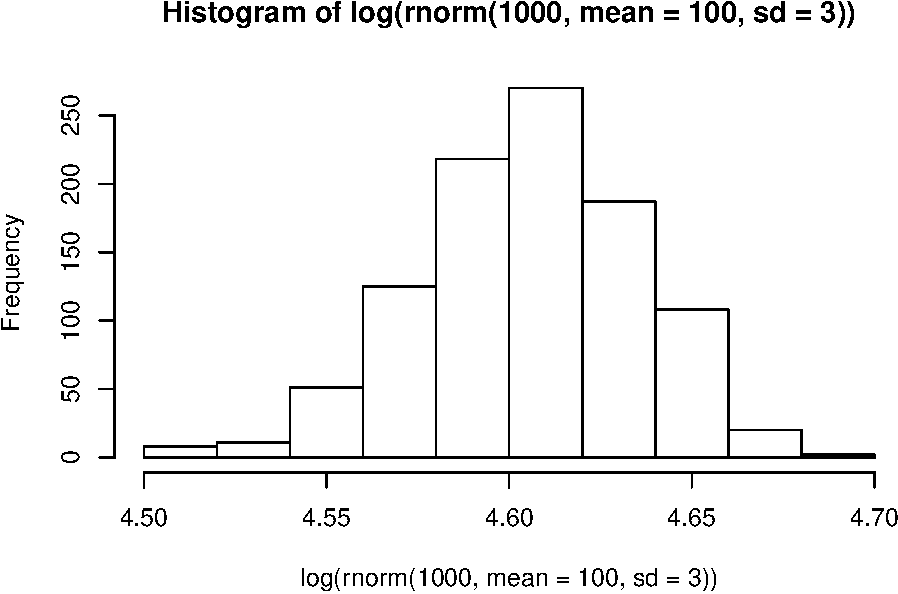
\includegraphics{R_tidyverse_for_geographers_files/figure-latex/unnamed-chunk-2-1.pdf}

\hypertarget{pipe-way}{%
\section{pipe way}\label{pipe-way}}

\begin{itemize}
\tightlist
\item
  Here you can linearly read the chain of operations
\end{itemize}

\begin{Shaded}
\begin{Highlighting}[]
\CommentTok{#  vector object            -> function -> function}
\KeywordTok{rnorm}\NormalTok{(}\DecValTok{1000}\NormalTok{, }\DataTypeTok{mean=}\DecValTok{100}\NormalTok{, }\DataTypeTok{sd=}\DecValTok{3}\NormalTok{) }\OperatorTok\StringTok{ }\KeywordTok{log}\NormalTok{() }\OperatorTok\StringTok{ }\KeywordTok{hist}\NormalTok{()}
\end{Highlighting}
\end{Shaded}

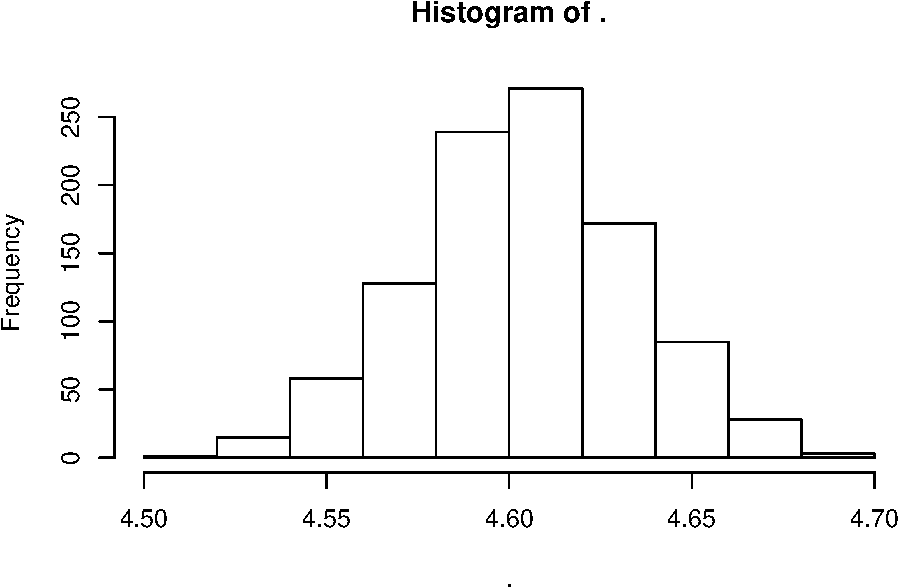
\includegraphics{R_tidyverse_for_geographers_files/figure-latex/unnamed-chunk-3-1.pdf}

\textbf{So pipes allow us to arbitrarily long things without nesting or
creating copyies of dataframes}

\begin{center}\rule{0.5\linewidth}{\linethickness}\end{center}

\hypertarget{life-before-and-after-dplyr}{%
\section{Life before and after
dplyr}\label{life-before-and-after-dplyr}}

\begin{itemize}
\tightlist
\item
  excellent tutorial:
  {[}\url{https://suzan.rbind.io/categories/tutorial/}{]}
\end{itemize}

\hypertarget{tibbles-vs-dataframes--}{%
\section{- Tibbles vs dataframes -}\label{tibbles-vs-dataframes--}}

\hypertarget{tibbles-are-a-more-clever-version-of-data-frames-that-offer-some-features-tibble}{%
\section{tibbles are a more clever version of data frames that offer
some features
(?tibble)}\label{tibbles-are-a-more-clever-version-of-data-frames-that-offer-some-features-tibble}}

\hypertarget{but-also-are-compatible-for-tidyverse-methods}{%
\section{but also, are compatible for tidyverse
methods}\label{but-also-are-compatible-for-tidyverse-methods}}

\begin{Shaded}
\begin{Highlighting}[]
\NormalTok{junk_df <-}\StringTok{ }\KeywordTok{data.frame}\NormalTok{(}\DataTypeTok{x=}\KeywordTok{rnorm}\NormalTok{(}\DecValTok{50}\NormalTok{, }\DataTypeTok{mean =} \DecValTok{0}\NormalTok{, }\DataTypeTok{sd=}\DecValTok{10}\NormalTok{), }
                   \DataTypeTok{y=}\KeywordTok{rnorm}\NormalTok{(}\DecValTok{50}\NormalTok{, }\DataTypeTok{mean=}\DecValTok{10}\NormalTok{, }\DataTypeTok{sd=}\DecValTok{1}\NormalTok{))}
\KeywordTok{print}\NormalTok{(junk_df) }\CommentTok{# prints the whole df!}
\end{Highlighting}
\end{Shaded}

\begin{verbatim}
##              x         y
## 1    1.7976335 10.505454
## 2   19.3920186  9.925693
## 3   -9.7786226  9.006092
## 4    1.5021817  9.240930
## 5  -14.7066993  9.723059
## 6   10.6792090  9.468869
## 7   -7.5120057  9.289074
## 8    6.1836787  8.590613
## 9    3.2696623 10.140312
## 10  -6.1224464 10.626501
## 11  13.8709901  9.017777
## 12 -15.2528043  8.765815
## 13  -5.8391234  8.956872
## 14  -3.9544170  9.534531
## 15   5.3844466  8.999447
## 16  10.8916225 10.603027
## 17 -22.2182978  9.493433
## 18  -1.1398281 10.049315
## 19   4.6414433  8.776759
## 20  -8.2120159 10.386167
## 21   4.8760902  7.861031
## 22  -2.6349752  8.903090
## 23  16.8497026 11.089865
## 24  -4.9384142 10.677672
## 25  -6.3287999 10.852870
## 26  17.0094790  9.912896
## 27  -0.3449704 10.022145
## 28  -6.5895266 10.396968
## 29 -11.2968547 10.480868
## 30  20.0826011  8.881388
## 31   6.5727024 10.837481
## 32   0.4510971  7.640171
## 33   8.2226437 11.867960
## 34  -1.6192400 10.748036
## 35   7.4469003  9.186233
## 36 -10.8109354 10.251924
## 37  20.1871763 10.864173
## 38   5.2483511 10.500143
## 39  -4.9226971 10.649579
## 40  -1.5537039  9.745509
## 41   7.1785737  9.526603
## 42   6.1186613  9.387935
## 43   5.7874680  9.346613
## 44  -1.3751109 10.122563
## 45   5.7936396 10.954642
## 46 -13.8797604 10.044760
## 47  -3.0867755  9.489731
## 48  -0.8850357 10.782255
## 49 -16.9082494  9.343850
## 50  -8.2148492  8.536392
\end{verbatim}

\begin{Shaded}
\begin{Highlighting}[]
\NormalTok{junk_tb <-}\StringTok{ }\KeywordTok{tibble}\NormalTok{(}\DataTypeTok{x=}\KeywordTok{rnorm}\NormalTok{(}\DecValTok{50}\NormalTok{, }\DataTypeTok{mean =} \DecValTok{0}\NormalTok{, }\DataTypeTok{sd=}\DecValTok{10}\NormalTok{), }
                      \DataTypeTok{y=}\KeywordTok{rnorm}\NormalTok{(}\DecValTok{50}\NormalTok{, }\DataTypeTok{mean=}\DecValTok{10}\NormalTok{, }\DataTypeTok{sd=}\DecValTok{1}\NormalTok{))}
\KeywordTok{print}\NormalTok{(junk_tb) }\CommentTok{# just prints the top 10 rows}
\end{Highlighting}
\end{Shaded}

\begin{verbatim}
## # A tibble: 50 x 2
##            x     y
##        <dbl> <dbl>
##  1  21.8     10.8 
##  2   2.60     9.89
##  3   4.44    10.0 
##  4   3.31    11.4 
##  5  -0.00197 11.4 
##  6 -12.3     10.7 
##  7   4.81    10.8 
##  8  -0.576   11.4 
##  9  15.7      9.38
## 10   3.07     9.47
## # ... with 40 more rows
\end{verbatim}

\hypertarget{filtering--}{%
\section{- Filtering -}\label{filtering--}}

\hypertarget{filtering-data-before-dplyr}{%
\section{filtering data before
dplyr:}\label{filtering-data-before-dplyr}}

\begin{Shaded}
\begin{Highlighting}[]
\NormalTok{iris[iris[,}\StringTok{'Species'}\NormalTok{]}\OperatorTok{==}\StringTok{"setosa"} \OperatorTok{&}\StringTok{ }\NormalTok{iris[,}\StringTok{"Sepal.Length"}\NormalTok{] }\OperatorTok{>}\StringTok{ }\FloatTok{5.0}\NormalTok{,]}
\end{Highlighting}
\end{Shaded}

\begin{verbatim}
##    Sepal.Length Sepal.Width Petal.Length Petal.Width Species
## 1           5.1         3.5          1.4         0.2  setosa
## 6           5.4         3.9          1.7         0.4  setosa
## 11          5.4         3.7          1.5         0.2  setosa
## 15          5.8         4.0          1.2         0.2  setosa
## 16          5.7         4.4          1.5         0.4  setosa
## 17          5.4         3.9          1.3         0.4  setosa
## 18          5.1         3.5          1.4         0.3  setosa
## 19          5.7         3.8          1.7         0.3  setosa
## 20          5.1         3.8          1.5         0.3  setosa
## 21          5.4         3.4          1.7         0.2  setosa
## 22          5.1         3.7          1.5         0.4  setosa
## 24          5.1         3.3          1.7         0.5  setosa
## 28          5.2         3.5          1.5         0.2  setosa
## 29          5.2         3.4          1.4         0.2  setosa
## 32          5.4         3.4          1.5         0.4  setosa
## 33          5.2         4.1          1.5         0.1  setosa
## 34          5.5         4.2          1.4         0.2  setosa
## 37          5.5         3.5          1.3         0.2  setosa
## 40          5.1         3.4          1.5         0.2  setosa
## 45          5.1         3.8          1.9         0.4  setosa
## 47          5.1         3.8          1.6         0.2  setosa
## 49          5.3         3.7          1.5         0.2  setosa
\end{verbatim}

\hypertarget{filtering-with-dplyr}{%
\section{filtering with dplyr}\label{filtering-with-dplyr}}

\begin{Shaded}
\begin{Highlighting}[]
\NormalTok{iris }\OperatorTok\StringTok{ }\KeywordTok{filter}\NormalTok{(Species}\OperatorTok{==}\StringTok{"setosa"} \OperatorTok{&}\StringTok{ }\NormalTok{Sepal.Length }\OperatorTok{>}\StringTok{ }\FloatTok{5.0}\NormalTok{)}
\end{Highlighting}
\end{Shaded}

\begin{verbatim}
##    Sepal.Length Sepal.Width Petal.Length Petal.Width Species
## 1           5.1         3.5          1.4         0.2  setosa
## 2           5.4         3.9          1.7         0.4  setosa
## 3           5.4         3.7          1.5         0.2  setosa
## 4           5.8         4.0          1.2         0.2  setosa
## 5           5.7         4.4          1.5         0.4  setosa
## 6           5.4         3.9          1.3         0.4  setosa
## 7           5.1         3.5          1.4         0.3  setosa
## 8           5.7         3.8          1.7         0.3  setosa
## 9           5.1         3.8          1.5         0.3  setosa
## 10          5.4         3.4          1.7         0.2  setosa
## 11          5.1         3.7          1.5         0.4  setosa
## 12          5.1         3.3          1.7         0.5  setosa
## 13          5.2         3.5          1.5         0.2  setosa
## 14          5.2         3.4          1.4         0.2  setosa
## 15          5.4         3.4          1.5         0.4  setosa
## 16          5.2         4.1          1.5         0.1  setosa
## 17          5.5         4.2          1.4         0.2  setosa
## 18          5.5         3.5          1.3         0.2  setosa
## 19          5.1         3.4          1.5         0.2  setosa
## 20          5.1         3.8          1.9         0.4  setosa
## 21          5.1         3.8          1.6         0.2  setosa
## 22          5.3         3.7          1.5         0.2  setosa
\end{verbatim}

\hypertarget{creating-or-transforming-variables--}{%
\section{- Creating or transforming variables
-}\label{creating-or-transforming-variables--}}

\begin{Shaded}
\begin{Highlighting}[]
\NormalTok{iris <-}\StringTok{ }\NormalTok{iris }\OperatorTok\StringTok{ }
\StringTok{  }\KeywordTok{mutate}\NormalTok{(}\DataTypeTok{p_wl_ratio =}\NormalTok{ Petal.Width}\OperatorTok{/}\NormalTok{Petal.Length) }\OperatorTok\StringTok{ }
\StringTok{  }\KeywordTok{mutate}\NormalTok{(}\DataTypeTok{narrow =} \KeywordTok{ifelse}\NormalTok{(p_wl_ratio }\OperatorTok{<}\StringTok{ }\FloatTok{0.25}\NormalTok{, }\OtherTok{TRUE}\NormalTok{, }\OtherTok{FALSE}\NormalTok{))}
\end{Highlighting}
\end{Shaded}

\hypertarget{renaming-variables--}{%
\section{- Renaming variables -}\label{renaming-variables--}}

\begin{Shaded}
\begin{Highlighting}[]
\NormalTok{iris }\OperatorTok\StringTok{ }\KeywordTok{names}\NormalTok{()}
\end{Highlighting}
\end{Shaded}

\begin{verbatim}
## [1] "Sepal.Length" "Sepal.Width"  "Petal.Length" "Petal.Width" 
## [5] "Species"      "p_wl_ratio"   "narrow"
\end{verbatim}

\begin{Shaded}
\begin{Highlighting}[]
\NormalTok{iris }\OperatorTok\StringTok{ }
\StringTok{  }\KeywordTok{rename_all}\NormalTok{(tolower) }\OperatorTok\StringTok{ }\CommentTok{# rename cols with lowercase}
\StringTok{  }\KeywordTok{head}\NormalTok{()}
\end{Highlighting}
\end{Shaded}

\begin{verbatim}
##   sepal.length sepal.width petal.length petal.width species p_wl_ratio
## 1          5.1         3.5          1.4         0.2  setosa  0.1428571
## 2          4.9         3.0          1.4         0.2  setosa  0.1428571
## 3          4.7         3.2          1.3         0.2  setosa  0.1538462
## 4          4.6         3.1          1.5         0.2  setosa  0.1333333
## 5          5.0         3.6          1.4         0.2  setosa  0.1428571
## 6          5.4         3.9          1.7         0.4  setosa  0.2352941
##   narrow
## 1   TRUE
## 2   TRUE
## 3   TRUE
## 4   TRUE
## 5   TRUE
## 6   TRUE
\end{verbatim}

\hypertarget{sample-random-rows--}{%
\section{- sample random rows -}\label{sample-random-rows--}}

\begin{Shaded}
\begin{Highlighting}[]
\NormalTok{iris }\OperatorTok\StringTok{ }
\StringTok{  }\KeywordTok{sample_n}\NormalTok{(}\DecValTok{10}\NormalTok{)}
\end{Highlighting}
\end{Shaded}

\begin{verbatim}
##     Sepal.Length Sepal.Width Petal.Length Petal.Width    Species
## 59           6.6         2.9          4.6         1.3 versicolor
## 28           5.2         3.5          1.5         0.2     setosa
## 30           4.7         3.2          1.6         0.2     setosa
## 77           6.8         2.8          4.8         1.4 versicolor
## 76           6.6         3.0          4.4         1.4 versicolor
## 84           6.0         2.7          5.1         1.6 versicolor
## 141          6.7         3.1          5.6         2.4  virginica
## 125          6.7         3.3          5.7         2.1  virginica
## 94           5.0         2.3          3.3         1.0 versicolor
## 124          6.3         2.7          4.9         1.8  virginica
##     p_wl_ratio narrow
## 59   0.2826087  FALSE
## 28   0.1333333   TRUE
## 30   0.1250000   TRUE
## 77   0.2916667  FALSE
## 76   0.3181818  FALSE
## 84   0.3137255  FALSE
## 141  0.4285714  FALSE
## 125  0.3684211  FALSE
## 94   0.3030303  FALSE
## 124  0.3673469  FALSE
\end{verbatim}

\hypertarget{summarize-groups-with-a-statistic--}{%
\section{- Summarize groups with a statistic
-}\label{summarize-groups-with-a-statistic--}}

\begin{Shaded}
\begin{Highlighting}[]
\NormalTok{iris }\OperatorTok\StringTok{ }\CommentTok{# count number of observations per species}
\StringTok{  }\KeywordTok{group_by}\NormalTok{(Species) }\OperatorTok\StringTok{ }
\StringTok{  }\KeywordTok{summarize}\NormalTok{(}\DataTypeTok{nobs =} \KeywordTok{n}\NormalTok{()) }\OperatorTok\StringTok{ }
\StringTok{  }\KeywordTok{ungroup}\NormalTok{()}
\end{Highlighting}
\end{Shaded}

\begin{verbatim}
## # A tibble: 3 x 2
##   Species     nobs
##   <fct>      <int>
## 1 setosa        50
## 2 versicolor    50
## 3 virginica     50
\end{verbatim}

\begin{Shaded}
\begin{Highlighting}[]
\NormalTok{iris }\OperatorTok\StringTok{ }\CommentTok{# calc mean of traits per species}
\StringTok{  }\KeywordTok{group_by}\NormalTok{(Species) }\OperatorTok\StringTok{ }
\StringTok{  }\KeywordTok{summarise_all}\NormalTok{(mean)}
\end{Highlighting}
\end{Shaded}

\begin{verbatim}
## # A tibble: 3 x 7
##   Species    Sepal.Length Sepal.Width Petal.Length Petal.Width p_wl_ratio
##   <fct>             <dbl>       <dbl>        <dbl>       <dbl>      <dbl>
## 1 setosa             5.01        3.43         1.46       0.246      0.168
## 2 versicolor         5.94        2.77         4.26       1.33       0.311
## 3 virginica          6.59        2.97         5.55       2.03       0.367
## # ... with 1 more variable: narrow <dbl>
\end{verbatim}

\begin{Shaded}
\begin{Highlighting}[]
\NormalTok{iris }\OperatorTok\StringTok{ }\CommentTok{# calc mean of traits across three species}
\StringTok{  }\KeywordTok{group_by}\NormalTok{(Species) }\OperatorTok\StringTok{ }
\StringTok{  }\KeywordTok{summarise_all}\NormalTok{(mean) }\OperatorTok\StringTok{ }
\StringTok{  }\KeywordTok{ungroup}\NormalTok{() }\OperatorTok\StringTok{ }
\StringTok{  }\KeywordTok{select}\NormalTok{(}\OperatorTok{-}\NormalTok{Species) }\OperatorTok\StringTok{ }
\StringTok{  }\KeywordTok{summarize_all}\NormalTok{(mean)}
\end{Highlighting}
\end{Shaded}

\begin{verbatim}
## # A tibble: 1 x 6
##   Sepal.Length Sepal.Width Petal.Length Petal.Width p_wl_ratio narrow
##          <dbl>       <dbl>        <dbl>       <dbl>      <dbl>  <dbl>
## 1         5.84        3.06         3.76        1.20      0.282  0.293
\end{verbatim}

\hypertarget{readr-tidyr-for-getting-data-into-a-workable-shape--}{%
\section{readr \& tidyr for getting data into a workable shape
----------------------------}\label{readr-tidyr-for-getting-data-into-a-workable-shape--}}

\begin{Shaded}
\begin{Highlighting}[]
\KeywordTok{read.table}\NormalTok{(}\StringTok{"data/mei_1950_2018.data"}\NormalTok{,}\DataTypeTok{skip =} \DecValTok{1}\NormalTok{, }\DataTypeTok{nrows =} \DecValTok{68}\NormalTok{) }\CommentTok{# base R way}
\end{Highlighting}
\end{Shaded}

\begin{verbatim}
##      V1     V2     V3     V4     V5     V6     V7     V8     V9    V10
## 1  1950 -1.062 -1.163 -1.312 -1.098 -1.433 -1.391 -1.296 -1.053 -0.634
## 2  1951 -1.070 -1.183 -1.204 -0.544 -0.360  0.349  0.666  0.829  0.743
## 3  1952  0.419  0.117  0.047  0.198 -0.309 -0.723 -0.316 -0.378  0.313
## 4  1953  0.030  0.377  0.257  0.668  0.784  0.218  0.368  0.213  0.501
## 5  1954 -0.051 -0.048  0.147 -0.634 -1.416 -1.564 -1.378 -1.471 -1.166
## 6  1955 -0.762 -0.697 -1.147 -1.662 -1.642 -2.243 -1.998 -2.073 -1.823
## 7  1956 -1.437 -1.303 -1.399 -1.248 -1.317 -1.502 -1.259 -1.131 -1.359
## 8  1957 -0.941 -0.372  0.101  0.372  0.866  0.769  0.908  1.148  1.125
## 9  1958  1.472  1.439  1.320  0.987  0.719  0.864  0.693  0.427  0.188
## 10 1959  0.548  0.796  0.495  0.192  0.013 -0.018 -0.134  0.114  0.105
## 11 1960 -0.299 -0.274 -0.094 -0.005 -0.335 -0.254 -0.340 -0.251 -0.465
## 12 1961 -0.163 -0.257 -0.088  0.004 -0.288 -0.137 -0.216 -0.304 -0.301
## 13 1962 -1.087 -0.988 -0.712 -1.068 -0.910 -0.852 -0.701 -0.543 -0.551
## 14 1963 -0.739 -0.863 -0.690 -0.768 -0.477 -0.087  0.401  0.597  0.750
## 15 1964  0.874  0.468 -0.269 -0.562 -1.242 -1.115 -1.405 -1.503 -1.311
## 16 1965 -0.557 -0.353 -0.278  0.063  0.490  0.915  1.360  1.443  1.406
## 17 1966  1.306  1.170  0.681  0.506 -0.152 -0.168 -0.136  0.155 -0.085
## 18 1967 -0.473 -0.919 -1.066 -1.037 -0.455 -0.266 -0.521 -0.395 -0.621
## 19 1968 -0.619 -0.749 -0.641 -0.959 -1.095 -0.771 -0.527 -0.102  0.220
## 20 1969  0.664  0.833  0.453  0.616  0.696  0.820  0.467  0.218  0.177
## 21 1970  0.372  0.415  0.220  0.000 -0.126 -0.659 -1.089 -1.016 -1.252
## 22 1971 -1.223 -1.528 -1.817 -1.870 -1.464 -1.448 -1.230 -1.225 -1.460
## 23 1972 -0.596 -0.424 -0.269 -0.171  0.464  1.069  1.827  1.821  1.558
## 24 1973  1.726  1.500  0.860  0.473 -0.106 -0.769 -1.081 -1.347 -1.727
## 25 1974 -1.939 -1.793 -1.767 -1.643 -1.077 -0.670 -0.769 -0.671 -0.627
## 26 1975 -0.538 -0.600 -0.879 -0.959 -0.863 -1.150 -1.519 -1.730 -1.874
## 27 1976 -1.610 -1.392 -1.234 -1.180 -0.496  0.307  0.615  0.664  1.038
## 28 1977  0.521  0.273  0.139  0.545  0.326  0.451  0.866  0.695  0.800
## 29 1978  0.773  0.899  0.936  0.191 -0.388 -0.579 -0.433 -0.200 -0.389
## 30 1979  0.600  0.362 -0.010  0.292  0.380  0.423  0.369  0.625  0.786
## 31 1980  0.672  0.585  0.689  0.927  0.961  0.907  0.749  0.336  0.281
## 32 1981 -0.262 -0.151  0.456  0.671  0.161 -0.019 -0.048 -0.088  0.187
## 33 1982 -0.270 -0.137  0.103  0.013  0.429  0.944  1.604  1.799  1.811
## 34 1983  2.683  2.910  3.012  2.808  2.542  2.240  1.763  1.178  0.497
## 35 1984 -0.330 -0.529  0.139  0.373  0.131 -0.079 -0.084 -0.154 -0.106
## 36 1985 -0.561 -0.595 -0.709 -0.472 -0.707 -0.133 -0.143 -0.367 -0.526
## 37 1986 -0.301 -0.195  0.028 -0.099  0.350  0.306  0.383  0.775  1.088
## 38 1987  1.250  1.205  1.722  1.859  2.140  1.964  1.859  1.999  1.894
## 39 1988  1.119  0.706  0.491  0.387  0.119 -0.622 -1.145 -1.303 -1.506
## 40 1989 -1.120 -1.262 -1.054 -0.763 -0.435 -0.253 -0.459 -0.497 -0.311
## 41 1990  0.237  0.563  0.956  0.469  0.637  0.484  0.120  0.131  0.378
## 42 1991  0.313  0.314  0.402  0.454  0.759  1.100  1.023  1.024  0.760
## 43 1992  1.743  1.870  1.991  2.258  2.129  1.748  1.018  0.570  0.497
## 44 1993  0.687  0.974  0.990  1.417  1.998  1.591  1.170  1.042  0.992
## 45 1994  0.353  0.182  0.157  0.473  0.573  0.788  0.880  0.773  0.908
## 46 1995  1.220  0.946  0.853  0.469  0.563  0.508  0.207 -0.143 -0.426
## 47 1996 -0.612 -0.580 -0.238 -0.386 -0.127  0.068 -0.204 -0.374 -0.437
## 48 1997 -0.490 -0.621 -0.252  0.543  1.165  2.292  2.805  3.040  3.044
## 49 1998  2.466  2.761  2.755  2.661  2.212  1.292  0.347 -0.331 -0.600
## 50 1999 -1.053 -1.140 -0.971 -0.903 -0.660 -0.361 -0.507 -0.745 -0.953
## 51 2000 -1.139 -1.210 -1.113 -0.409  0.169 -0.053 -0.184 -0.145 -0.227
## 52 2001 -0.505 -0.661 -0.560 -0.055  0.233  0.006  0.270  0.338 -0.165
## 53 2002  0.009 -0.171 -0.121  0.414  0.851  0.913  0.685  1.017  0.908
## 54 2003  1.218  0.935  0.833  0.421  0.111  0.097  0.144  0.316  0.477
## 55 2004  0.327  0.359 -0.035  0.374  0.539  0.267  0.541  0.627  0.572
## 56 2005  0.320  0.810  1.067  0.637  0.836  0.585  0.490  0.352  0.315
## 57 2006 -0.438 -0.424 -0.527 -0.575  0.008  0.530  0.691  0.759  0.823
## 58 2007  0.985  0.528  0.120  0.020  0.247 -0.215 -0.288 -0.441 -1.181
## 59 2008 -1.020 -1.388 -1.579 -0.879 -0.368  0.133  0.054 -0.266 -0.551
## 60 2009 -0.726 -0.707 -0.723 -0.105  0.361  0.819  1.035  1.067  0.735
## 61 2010  1.067  1.520  1.469  0.990  0.643 -0.325 -1.156 -1.683 -1.868
## 62 2011 -1.739 -1.563 -1.575 -1.399 -0.288 -0.075 -0.228 -0.519 -0.769
## 63 2012 -0.993 -0.695 -0.398  0.112  0.747  0.835  1.098  0.619  0.339
## 64 2013  0.096 -0.080 -0.037  0.095  0.146 -0.168 -0.355 -0.480 -0.133
## 65 2014 -0.275 -0.266  0.027  0.312  0.976  0.980  0.882  0.954  0.585
## 66 2015  0.420  0.459  0.631  0.943  1.584  2.045  1.948  2.366  2.530
## 67 2016  2.227  2.169  1.984  2.124  1.699  1.001  0.312  0.175 -0.101
## 68 2017 -0.055 -0.056 -0.080  0.770  1.455  1.049  0.461  0.027 -0.449
##       V11    V12    V13
## 1  -0.433 -1.165 -1.261
## 2   0.736  0.703  0.478
## 3   0.275 -0.349 -0.124
## 4   0.093  0.075  0.324
## 5  -1.348 -1.140 -1.113
## 6  -1.753 -1.841 -1.877
## 7  -1.486 -1.038 -1.022
## 8   1.083  1.148  1.248
## 9   0.213  0.486  0.671
## 10 -0.060 -0.170 -0.261
## 11 -0.355 -0.331 -0.417
## 12 -0.539 -0.436 -0.634
## 13 -0.670 -0.623 -0.505
## 14  0.814  0.844  0.744
## 15 -1.225 -1.239 -0.936
## 16  1.219  1.362  1.252
## 17 -0.044  0.004 -0.199
## 18 -0.683 -0.426 -0.378
## 19  0.435  0.586  0.347
## 20  0.511  0.666  0.398
## 21 -1.088 -1.084 -1.223
## 22 -1.421 -1.329 -0.993
## 23  1.643  1.726  1.766
## 24 -1.667 -1.503 -1.848
## 25 -1.052 -1.251 -0.905
## 26 -1.987 -1.773 -1.757
## 27  0.946  0.493  0.550
## 28  0.986  0.975  0.860
## 29 -0.020  0.186  0.388
## 30  0.678  0.746  0.989
## 31  0.201  0.251  0.089
## 32  0.112 -0.038 -0.141
## 33  2.024  2.428  2.411
## 34  0.038 -0.132 -0.188
## 35  0.001 -0.352 -0.603
## 36 -0.139 -0.059 -0.293
## 37  0.979  0.873  1.190
## 38  1.647  1.271  1.282
## 39 -1.326 -1.468 -1.328
## 40 -0.341 -0.073  0.115
## 41  0.285  0.389  0.348
## 42  1.009  1.189  1.320
## 43  0.641  0.582  0.648
## 44  1.069  0.834  0.589
## 45  1.407  1.299  1.237
## 46 -0.477 -0.478 -0.554
## 47 -0.349 -0.146 -0.336
## 48  2.401  2.542  2.335
## 49 -0.798 -1.086 -0.922
## 50 -0.973 -1.050 -1.161
## 51 -0.387 -0.714 -0.566
## 52 -0.275 -0.153  0.019
## 53  1.000  1.090  1.145
## 54  0.516  0.570  0.351
## 55  0.508  0.805  0.667
## 56 -0.167 -0.392 -0.570
## 57  0.955  1.286  0.951
## 58 -1.217 -1.165 -1.193
## 59 -0.692 -0.597 -0.663
## 60  0.909  1.121  1.045
## 61 -1.899 -1.490 -1.577
## 62 -0.933 -0.949 -0.957
## 63  0.081  0.125  0.094
## 64  0.130 -0.053 -0.248
## 65  0.438  0.763  0.558
## 66  2.241  2.297  2.112
## 67 -0.379 -0.212 -0.121
## 68 -0.551 -0.277 -0.576
\end{verbatim}

\begin{Shaded}
\begin{Highlighting}[]
\NormalTok{mei_wide <-}\StringTok{ }\NormalTok{readr}\OperatorTok{::}\KeywordTok{read_table}\NormalTok{(}\StringTok{"data/mei_1950_2018.data"}\NormalTok{, }\DataTypeTok{skip =} \DecValTok{1}\NormalTok{, }\DataTypeTok{col_names =}\NormalTok{ F, }\DataTypeTok{n_max =} \DecValTok{68}\NormalTok{) }\CommentTok{# slightly easier tidyverse way}
\end{Highlighting}
\end{Shaded}

\begin{verbatim}
## Parsed with column specification:
## cols(
##   X1 = col_integer(),
##   X2 = col_double(),
##   X3 = col_double(),
##   X4 = col_double(),
##   X5 = col_double(),
##   X6 = col_double(),
##   X7 = col_double(),
##   X8 = col_double(),
##   X9 = col_double(),
##   X10 = col_double(),
##   X11 = col_double(),
##   X12 = col_double(),
##   X13 = col_double()
## )
\end{verbatim}

\begin{Shaded}
\begin{Highlighting}[]
\KeywordTok{names}\NormalTok{(mei_wide) <-}\StringTok{ }\KeywordTok{c}\NormalTok{(}\StringTok{"year"}\NormalTok{,}\DecValTok{1}\OperatorTok{:}\DecValTok{12}\NormalTok{) }\CommentTok{# add names to columns}

\NormalTok{mei_long <-}\StringTok{ }\NormalTok{mei_wide }\OperatorTok\StringTok{ }\CommentTok{# reshape the data frame from 'wide' to 'long' }
\StringTok{  }\KeywordTok{gather}\NormalTok{(}\DataTypeTok{key=}\StringTok{"month"}\NormalTok{,}\DataTypeTok{value=}\StringTok{"index"}\NormalTok{,}\OperatorTok{-}\NormalTok{year) }\OperatorTok\StringTok{ }\CommentTok{# use gather() to assemble key-value pairs}
\StringTok{  }\KeywordTok{mutate}\NormalTok{(}\DataTypeTok{date=}\KeywordTok{parse_date_time}\NormalTok{(}\KeywordTok{paste}\NormalTok{(year,month,}\DecValTok{1}\NormalTok{),}\StringTok{"ymd"}\NormalTok{)) }\CommentTok{# mutate the date}

\NormalTok{mei_long }\OperatorTok\StringTok{ }
\StringTok{  }\KeywordTok{ggplot}\NormalTok{(}\DataTypeTok{data=}\NormalTok{., }\KeywordTok{aes}\NormalTok{(date, index))}\OperatorTok{+}\KeywordTok{geom_line}\NormalTok{()}
\end{Highlighting}
\end{Shaded}

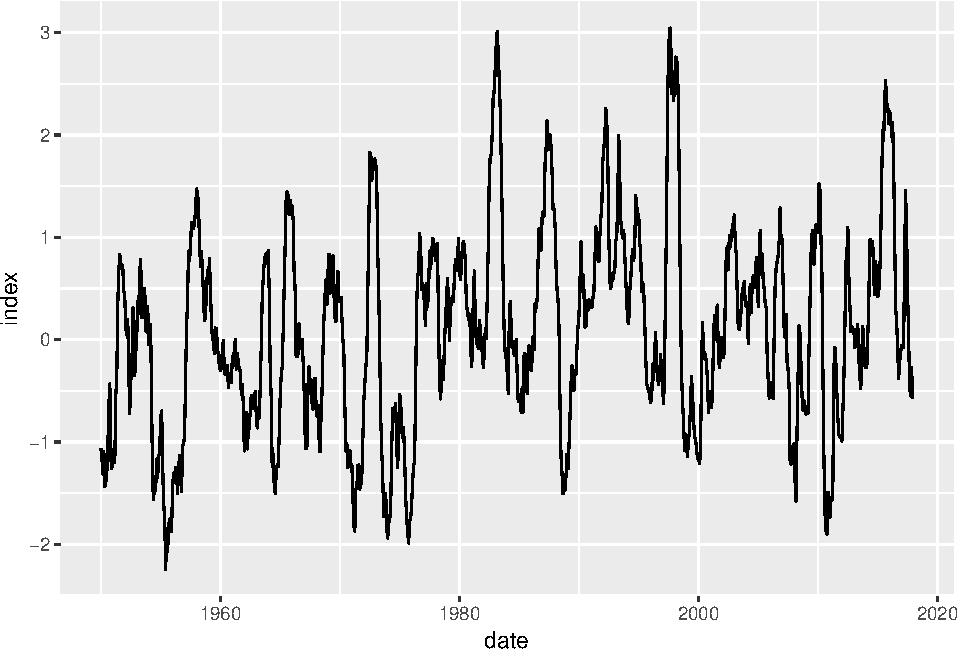
\includegraphics{R_tidyverse_for_geographers_files/figure-latex/unnamed-chunk-13-1.pdf}

\hypertarget{ggplotting-el-nino}{%
\section{ggPlotting El Niño
--------------------------------------------------------}\label{ggplotting-el-nino}}

\hypertarget{always-plot-your-data}{%
\section{``always plot your data''}\label{always-plot-your-data}}

\begin{Shaded}
\begin{Highlighting}[]
\NormalTok{tmp <-}\StringTok{ }\KeywordTok{read_csv}\NormalTok{(}\StringTok{"data/nino34_1870_2017.csv"}\NormalTok{)}
\end{Highlighting}
\end{Shaded}

\begin{verbatim}
## Parsed with column specification:
## cols(
##   year = col_integer(),
##   month = col_character(),
##   index = col_double(),
##   date = col_datetime(format = "")
## )
\end{verbatim}

\begin{Shaded}
\begin{Highlighting}[]
\CommentTok{# plot the whole record}
\NormalTok{tmp }\OperatorTok\StringTok{ }
\StringTok{  }\CommentTok{#__________________x_____y_______thing to add to plot}
\StringTok{  }\KeywordTok{ggplot}\NormalTok{(}\DataTypeTok{data=}\NormalTok{., }\KeywordTok{aes}\NormalTok{(date, index))}\OperatorTok{+}\KeywordTok{geom_line}\NormalTok{()}
\end{Highlighting}
\end{Shaded}

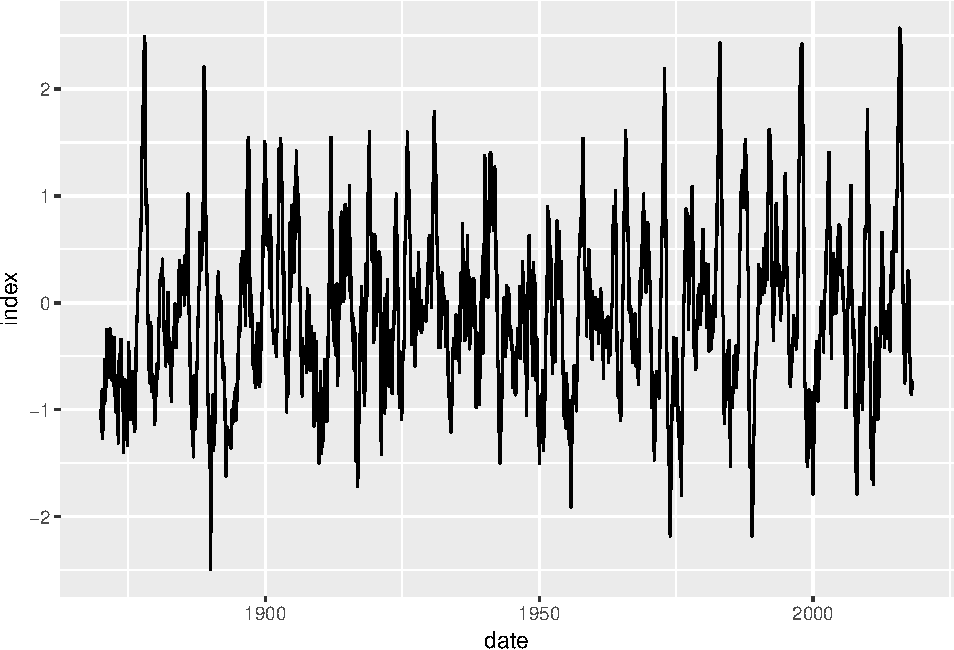
\includegraphics{R_tidyverse_for_geographers_files/figure-latex/unnamed-chunk-14-1.pdf}

\begin{Shaded}
\begin{Highlighting}[]
\CommentTok{#plot record by month}
\NormalTok{tmp }\OperatorTok
\StringTok{  }\KeywordTok{ggplot}\NormalTok{(}\DataTypeTok{data=}\NormalTok{., }\KeywordTok{aes}\NormalTok{(date, index))}\OperatorTok{+}
\StringTok{  }\KeywordTok{geom_line}\NormalTok{()}\OperatorTok{+}
\StringTok{  }\KeywordTok{geom_smooth}\NormalTok{(}\DataTypeTok{method=}\StringTok{'lm'}\NormalTok{,}\DataTypeTok{se=}\NormalTok{F)}\OperatorTok{+}
\StringTok{  }\KeywordTok{facet_wrap}\NormalTok{(}\OperatorTok{~}\NormalTok{month)}
\end{Highlighting}
\end{Shaded}

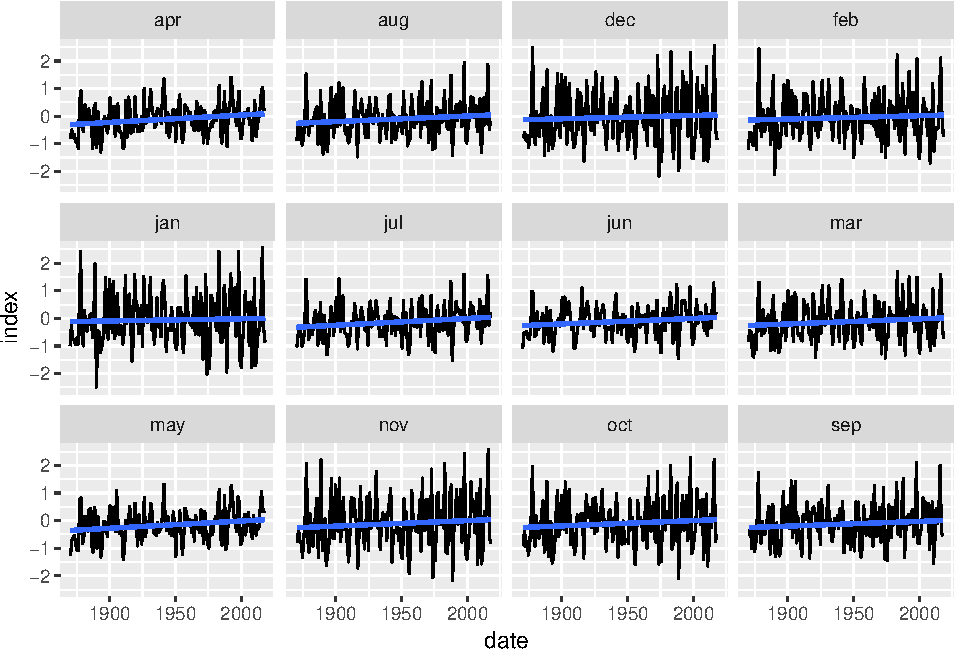
\includegraphics{R_tidyverse_for_geographers_files/figure-latex/unnamed-chunk-14-2.pdf}

\begin{Shaded}
\begin{Highlighting}[]
\CommentTok{# plot recent ENSO record}
\NormalTok{tmp }\OperatorTok
\StringTok{  }\KeywordTok{filter}\NormalTok{(year}\OperatorTok{>=}\DecValTok{1990}\NormalTok{) }\OperatorTok\StringTok{ }
\StringTok{  }\KeywordTok{ggplot}\NormalTok{(}\DataTypeTok{data=}\NormalTok{., }\KeywordTok{aes}\NormalTok{(date, index))}\OperatorTok{+}
\StringTok{  }\KeywordTok{geom_line}\NormalTok{()}
\end{Highlighting}
\end{Shaded}

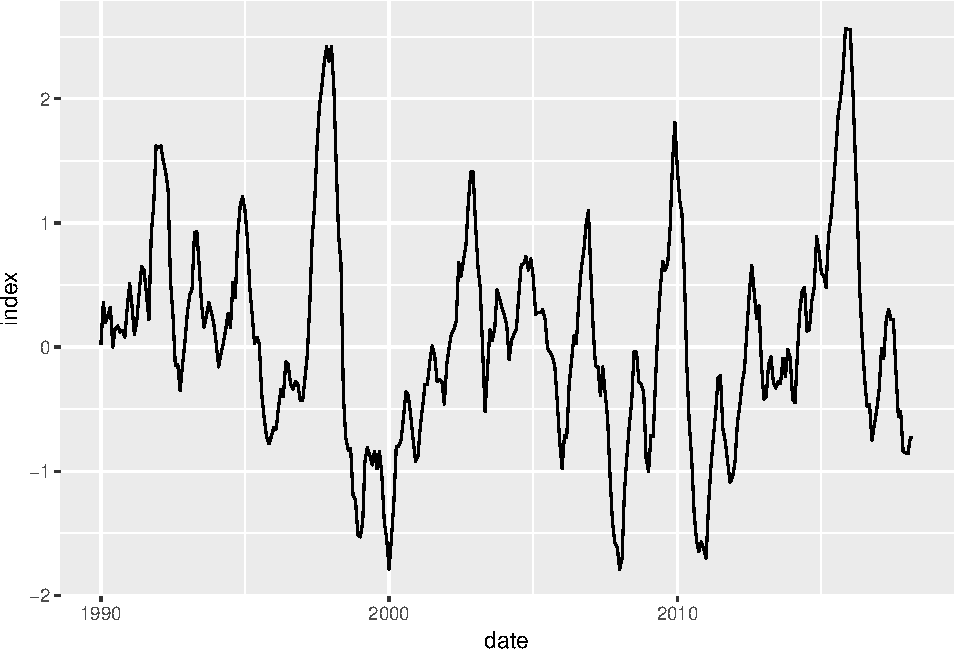
\includegraphics{R_tidyverse_for_geographers_files/figure-latex/unnamed-chunk-14-3.pdf}

\hypertarget{lets-smooth-the-record-with-a-moving-average}{%
\section{LETS `smooth' the record with a moving
average}\label{lets-smooth-the-record-with-a-moving-average}}

\begin{Shaded}
\begin{Highlighting}[]
\KeywordTok{library}\NormalTok{(RcppRoll)}
\NormalTok{tmp }\OperatorTok\StringTok{ }
\StringTok{  }\KeywordTok{arrange}\NormalTok{(date) }\OperatorTok\StringTok{ }
\StringTok{  }\KeywordTok{mutate}\NormalTok{(}\DataTypeTok{index_12mo =} \KeywordTok{roll_meanr}\NormalTok{(index, }\DataTypeTok{n=}\DecValTok{12}\NormalTok{, }\DataTypeTok{fill=}\OtherTok{NA}\NormalTok{)) }\OperatorTok\StringTok{  }\CommentTok{#}
\StringTok{  }\KeywordTok{filter}\NormalTok{(year}\OperatorTok{>=}\DecValTok{1990}\NormalTok{) }\OperatorTok\StringTok{ }
\StringTok{  }\KeywordTok{ggplot}\NormalTok{(}\DataTypeTok{data=}\NormalTok{., }\KeywordTok{aes}\NormalTok{(date, index))}\OperatorTok{+}
\StringTok{  }\KeywordTok{geom_line}\NormalTok{()}\OperatorTok{+}
\StringTok{  }\KeywordTok{geom_line}\NormalTok{(}\KeywordTok{aes}\NormalTok{(date, index_12mo),}\DataTypeTok{col=}\StringTok{'red'}\NormalTok{,}\DataTypeTok{lwd=}\FloatTok{1.5}\NormalTok{)}
\end{Highlighting}
\end{Shaded}

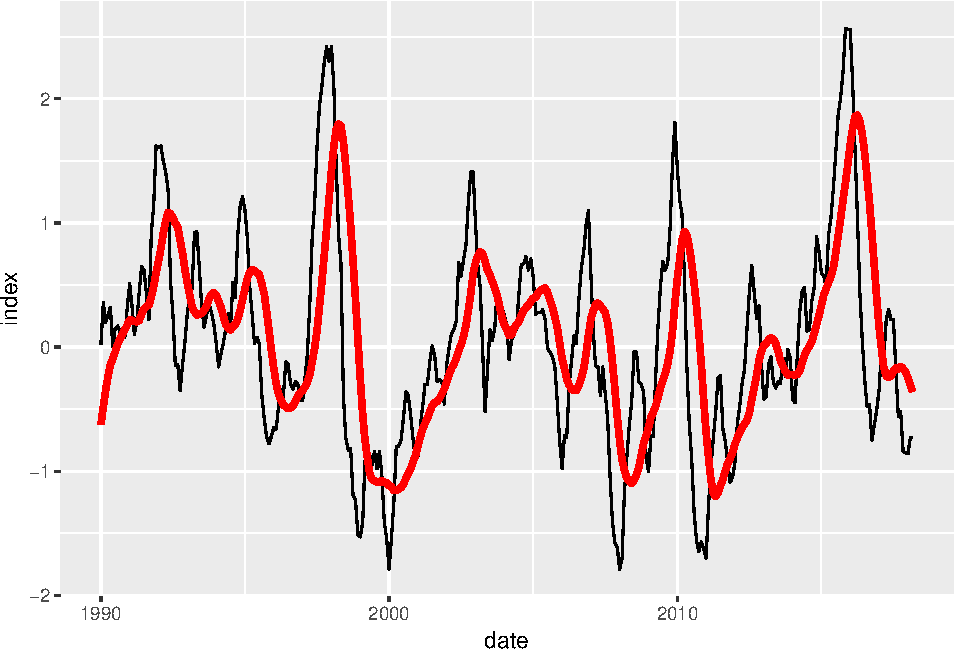
\includegraphics{R_tidyverse_for_geographers_files/figure-latex/unnamed-chunk-15-1.pdf}

\hypertarget{lets-deseasonlize-the-record-by-subtracting-the-monthly-mean}{%
\section{LET's `deseasonlize' the record by subtracting the monthly
mean}\label{lets-deseasonlize-the-record-by-subtracting-the-monthly-mean}}

\begin{Shaded}
\begin{Highlighting}[]
\NormalTok{df_norms <-}\StringTok{ }\NormalTok{tmp }\OperatorTok
\StringTok{  }\KeywordTok{group_by}\NormalTok{(month) }\OperatorTok\StringTok{ }
\StringTok{  }\KeywordTok{summarize}\NormalTok{(}\DataTypeTok{index_u =} \KeywordTok{mean}\NormalTok{(index, }\DataTypeTok{na.rm=}\NormalTok{T))}
\NormalTok{tmp2 <-}\StringTok{ }\KeywordTok{left_join}\NormalTok{(tmp, df_norms, }\DataTypeTok{by=}\KeywordTok{c}\NormalTok{(}\StringTok{"month"}\NormalTok{)) }\CommentTok{# now we join it back together}
\end{Highlighting}
\end{Shaded}

\begin{Shaded}
\begin{Highlighting}[]
\NormalTok{tmp2 }\OperatorTok\StringTok{ }
\StringTok{  }\KeywordTok{mutate}\NormalTok{(}\DataTypeTok{index_ds =}\NormalTok{ index}\OperatorTok{-}\NormalTok{index_u) }\OperatorTok\StringTok{ }
\StringTok{  }\KeywordTok{filter}\NormalTok{(year}\OperatorTok{>=}\DecValTok{1990}\NormalTok{) }\OperatorTok\StringTok{ }
\StringTok{  }\KeywordTok{ggplot}\NormalTok{(}\DataTypeTok{data=}\NormalTok{., }\KeywordTok{aes}\NormalTok{(date, index))}\OperatorTok{+}
\StringTok{  }\KeywordTok{geom_line}\NormalTok{()}\OperatorTok{+}
\StringTok{  }\KeywordTok{geom_line}\NormalTok{(}\KeywordTok{aes}\NormalTok{(date, index_ds), }\DataTypeTok{col=}\StringTok{'red'}\NormalTok{) }\CommentTok{# so that actually didn't make much of a difference}
\end{Highlighting}
\end{Shaded}

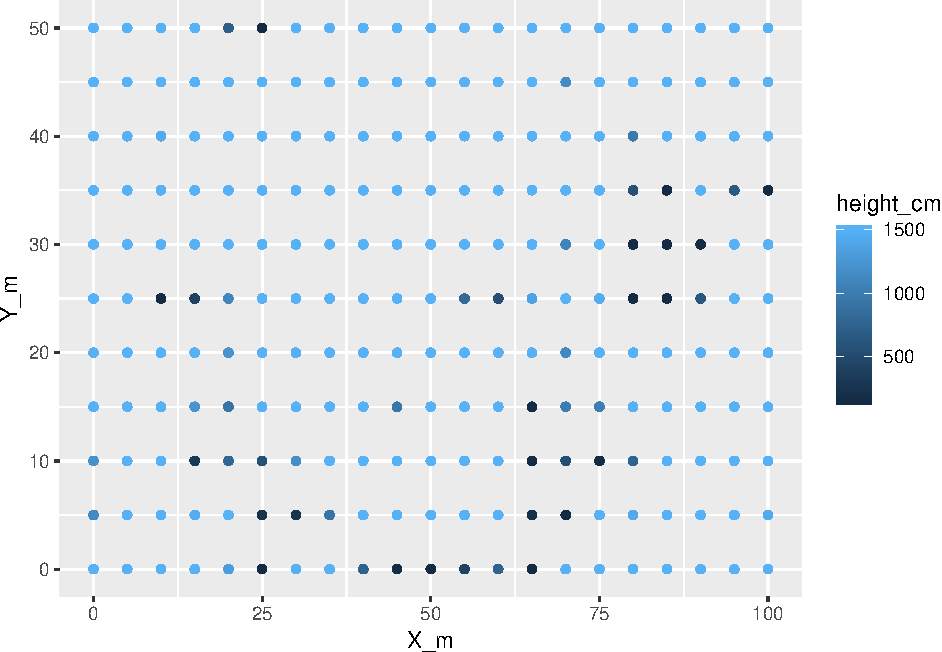
\includegraphics{R_tidyverse_for_geographers_files/figure-latex/unnamed-chunk-17-1.pdf}

\hypertarget{ggplot-spatial-data-la-selva-carbono-plots-data}{%
\section{ggplot spatial data: La Selva CARBONO plots data
---------------------------------------------}\label{ggplot-spatial-data-la-selva-carbono-plots-data}}

\begin{Shaded}
\begin{Highlighting}[]
\NormalTok{carb <-}\StringTok{ }\KeywordTok{read_csv}\NormalTok{(}\StringTok{"data/claros1999_2012fulldataset.csv"}\NormalTok{, }\DataTypeTok{skip =} \DecValTok{5}\NormalTok{)}
\end{Highlighting}
\end{Shaded}

\begin{verbatim}
## Parsed with column specification:
## cols(
##   `*Year` = col_integer(),
##   plot = col_character(),
##   Y_m = col_integer(),
##   X_m = col_integer(),
##   height_cm = col_integer(),
##   Date = col_character(),
##   Comments = col_character()
## )
\end{verbatim}

\begin{Shaded}
\begin{Highlighting}[]
\NormalTok{carb }\OperatorTok\StringTok{ }\KeywordTok{glimpse}\NormalTok{()}
\end{Highlighting}
\end{Shaded}

\begin{verbatim}
## Observations: 56,133
## Variables: 7
## $ `*Year`   <int> 1999, 1999, 1999, 1999, 1999, 1999, 1999, 1999, 1999...
## $ plot      <chr> "A1", "A1", "A1", "A1", "A1", "A1", "A1", "A1", "A1"...
## $ Y_m       <int> 15, 20, 30, 20, 0, 35, 30, 20, 25, 30, 30, 40, 25, 2...
## $ X_m       <int> 85, 10, 0, 100, 95, 45, 45, 65, 45, 100, 50, 15, 10,...
## $ height_cm <int> 150, 150, 150, 507, 579, 695, 712, 788, 811, 835, 83...
## $ Date      <chr> "12-Jul-99", "12-Jul-99", "12-Jul-99", "12-Jul-99", ...
## $ Comments  <chr> "Not done in 1999", "Not done in 1999", "Not done in...
\end{verbatim}

\begin{Shaded}
\begin{Highlighting}[]
\NormalTok{carb <-}\StringTok{ }\NormalTok{carb }\OperatorTok\StringTok{ }
\StringTok{  }\KeywordTok{rename}\NormalTok{(}\DataTypeTok{year=}\StringTok{`}\DataTypeTok{*Year}\StringTok{`}\NormalTok{) }\OperatorTok\StringTok{ }
\StringTok{  }\KeywordTok{mutate}\NormalTok{(}\DataTypeTok{date =} \KeywordTok{parse_date_time}\NormalTok{(Date, }\StringTok{'%d-%m-%y'}\NormalTok{)) }\OperatorTok\StringTok{ }
\StringTok{  }\KeywordTok{select}\NormalTok{(}\OperatorTok{-}\NormalTok{Date)}
\end{Highlighting}
\end{Shaded}

\begin{Shaded}
\begin{Highlighting}[]
\NormalTok{carb }\OperatorTok\StringTok{ }\CommentTok{# bad way}
\StringTok{  }\KeywordTok{filter}\NormalTok{(year}\OperatorTok{==}\DecValTok{1999}\NormalTok{) }\OperatorTok\StringTok{ }
\StringTok{  }\KeywordTok{ggplot}\NormalTok{(}\DataTypeTok{data=}\NormalTok{., }\KeywordTok{aes}\NormalTok{(X_m, Y_m, }\DataTypeTok{color=}\NormalTok{height_cm))}\OperatorTok{+}
\StringTok{  }\KeywordTok{geom_point}\NormalTok{()}
\end{Highlighting}
\end{Shaded}

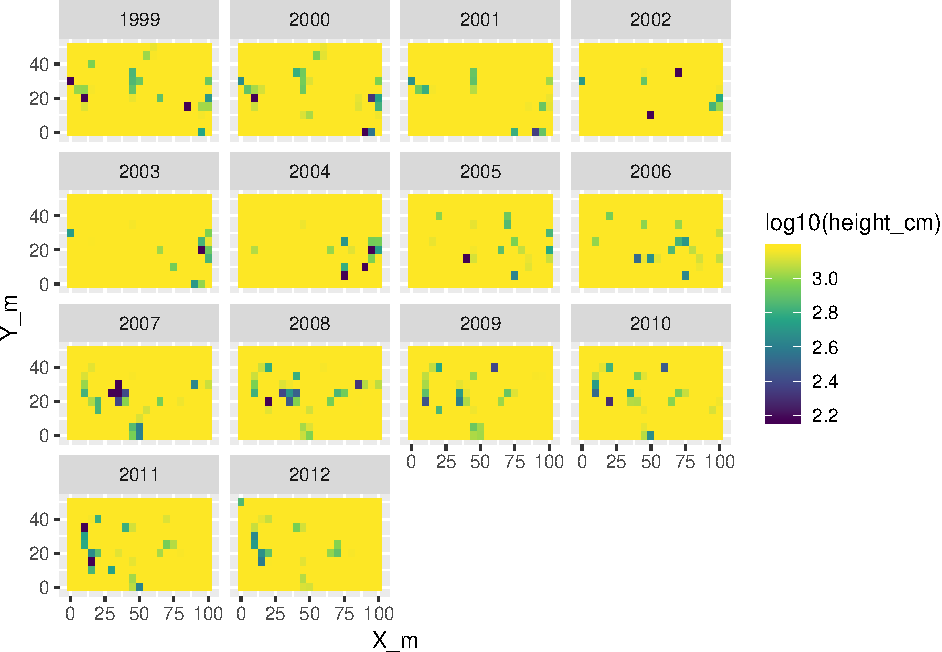
\includegraphics{R_tidyverse_for_geographers_files/figure-latex/unnamed-chunk-19-1.pdf}

\begin{Shaded}
\begin{Highlighting}[]
\NormalTok{carb }\OperatorTok\StringTok{ }\CommentTok{# better way}
\StringTok{  }\KeywordTok{filter}\NormalTok{(year}\OperatorTok{==}\DecValTok{1999} \OperatorTok{&}\StringTok{ }\NormalTok{plot}\OperatorTok{==}\StringTok{"A1"}\NormalTok{) }\OperatorTok\StringTok{ }
\StringTok{  }\KeywordTok{ggplot}\NormalTok{(}\DataTypeTok{data=}\NormalTok{., }\KeywordTok{aes}\NormalTok{(X_m, Y_m, }\DataTypeTok{fill=}\KeywordTok{log10}\NormalTok{(height_cm)))}\OperatorTok{+}
\StringTok{  }\KeywordTok{geom_raster}\NormalTok{()}\OperatorTok{+}
\StringTok{  }\KeywordTok{scale_fill_viridis_c}\NormalTok{()}
\end{Highlighting}
\end{Shaded}

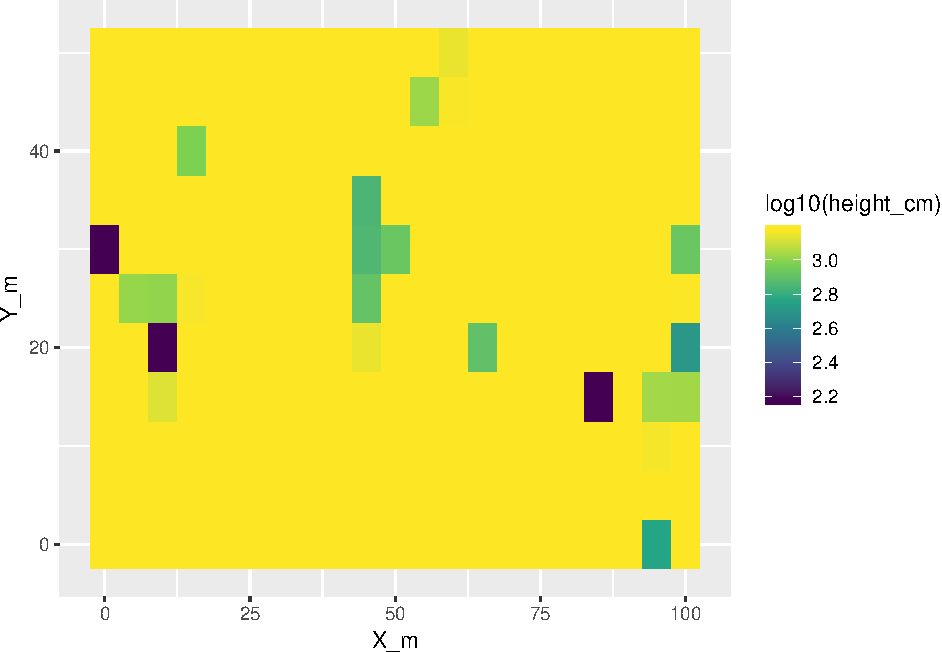
\includegraphics{R_tidyverse_for_geographers_files/figure-latex/unnamed-chunk-20-1.pdf}

\begin{Shaded}
\begin{Highlighting}[]
\NormalTok{carb }\OperatorTok\StringTok{ }\CommentTok{# visualize through time}
\StringTok{  }\KeywordTok{filter}\NormalTok{(plot}\OperatorTok{==}\StringTok{'A1'}\NormalTok{) }\OperatorTok
\StringTok{  }\KeywordTok{ggplot}\NormalTok{(}\DataTypeTok{data=}\NormalTok{., }\KeywordTok{aes}\NormalTok{(X_m, Y_m, }\DataTypeTok{fill=}\KeywordTok{log10}\NormalTok{(height_cm)))}\OperatorTok{+}
\StringTok{  }\KeywordTok{geom_raster}\NormalTok{()}\OperatorTok{+}
\StringTok{  }\KeywordTok{scale_fill_viridis_c}\NormalTok{()}\OperatorTok{+}
\StringTok{  }\KeywordTok{facet_wrap}\NormalTok{(}\OperatorTok{~}\NormalTok{year)}
\end{Highlighting}
\end{Shaded}

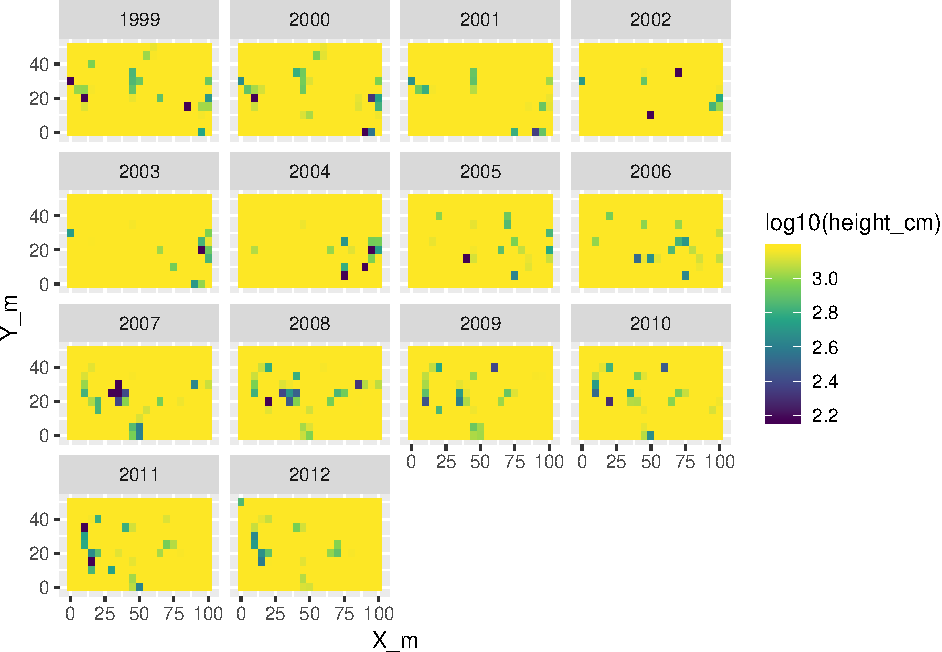
\includegraphics{R_tidyverse_for_geographers_files/figure-latex/unnamed-chunk-21-1.pdf}

\begin{Shaded}
\begin{Highlighting}[]
\CommentTok{#REALLY VISUALIZE it }
\KeywordTok{library}\NormalTok{(gganimate)}
\NormalTok{carb }\OperatorTok\StringTok{ }\CommentTok{# visualize through time}
\StringTok{  }\KeywordTok{filter}\NormalTok{(year}\OperatorTok{==}\DecValTok{1999}\NormalTok{) }\OperatorTok
\StringTok{  }\KeywordTok{ggplot}\NormalTok{(}\DataTypeTok{data=}\NormalTok{., }\KeywordTok{aes}\NormalTok{(X_m, Y_m, }\DataTypeTok{fill=}\KeywordTok{log10}\NormalTok{(height_cm)))}\OperatorTok{+}
\StringTok{  }\KeywordTok{geom_raster}\NormalTok{()}\OperatorTok{+}
\StringTok{  }\KeywordTok{scale_fill_viridis_c}\NormalTok{()}\OperatorTok{+}
\StringTok{  }\KeywordTok{facet_wrap}\NormalTok{(}\OperatorTok{~}\NormalTok{plot)}
\end{Highlighting}
\end{Shaded}

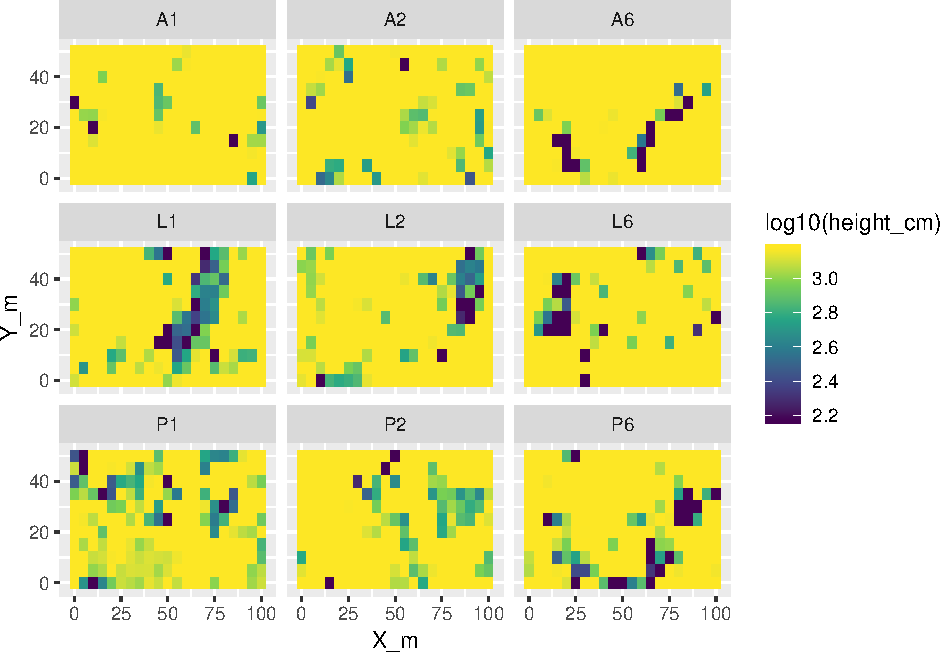
\includegraphics{R_tidyverse_for_geographers_files/figure-latex/unnamed-chunk-22-1.pdf}

\begin{Shaded}
\begin{Highlighting}[]
\KeywordTok{library}\NormalTok{(gganimate)}
\NormalTok{p <-}\StringTok{ }\NormalTok{carb }\OperatorTok\StringTok{ }\CommentTok{# visualize through time}
\StringTok{  }\KeywordTok{ggplot}\NormalTok{(}\DataTypeTok{data=}\NormalTok{., }\KeywordTok{aes}\NormalTok{(X_m, Y_m, }\DataTypeTok{fill=}\KeywordTok{log10}\NormalTok{(height_cm), }\DataTypeTok{frame=}\NormalTok{year))}\OperatorTok{+}
\StringTok{  }\KeywordTok{geom_raster}\NormalTok{()}\OperatorTok{+}
\StringTok{  }\KeywordTok{coord_equal}\NormalTok{()}\OperatorTok{+}
\StringTok{  }\KeywordTok{scale_fill_viridis_c}\NormalTok{(}\StringTok{"Canopy Height [log cm]"}\NormalTok{, }\DataTypeTok{option =} \StringTok{'B'}\NormalTok{)}\OperatorTok{+}
\StringTok{  }\KeywordTok{facet_wrap}\NormalTok{(}\OperatorTok{~}\NormalTok{plot)}\OperatorTok{+}
\StringTok{  }\KeywordTok{labs}\NormalTok{(}\DataTypeTok{title=}\StringTok{'Year: \{frame_time\}'}\NormalTok{)}
\KeywordTok{gganimate}\NormalTok{(p, }\StringTok{"outputs/carbono_plot_heights.gif"}\NormalTok{)}
\end{Highlighting}
\end{Shaded}

\begin{verbatim}
## Executing: 
## convert -loop 0 -delay 100 Rplot1.png Rplot2.png Rplot3.png
##     Rplot4.png Rplot5.png Rplot6.png Rplot7.png Rplot8.png
##     Rplot9.png Rplot10.png Rplot11.png Rplot12.png Rplot13.png
##     Rplot14.png 'carbono_plot_heights.gif'
\end{verbatim}

\begin{verbatim}
## Output at: carbono_plot_heights.gif
\end{verbatim}

\hypertarget{plot-distributions}{%
\section{Plot distributions
------------------------------------------------------}\label{plot-distributions}}

\begin{Shaded}
\begin{Highlighting}[]
\KeywordTok{hist}\NormalTok{(carb}\OperatorTok{$}\NormalTok{height_cm) }\CommentTok{# old base-R way to plot histogram}
\end{Highlighting}
\end{Shaded}

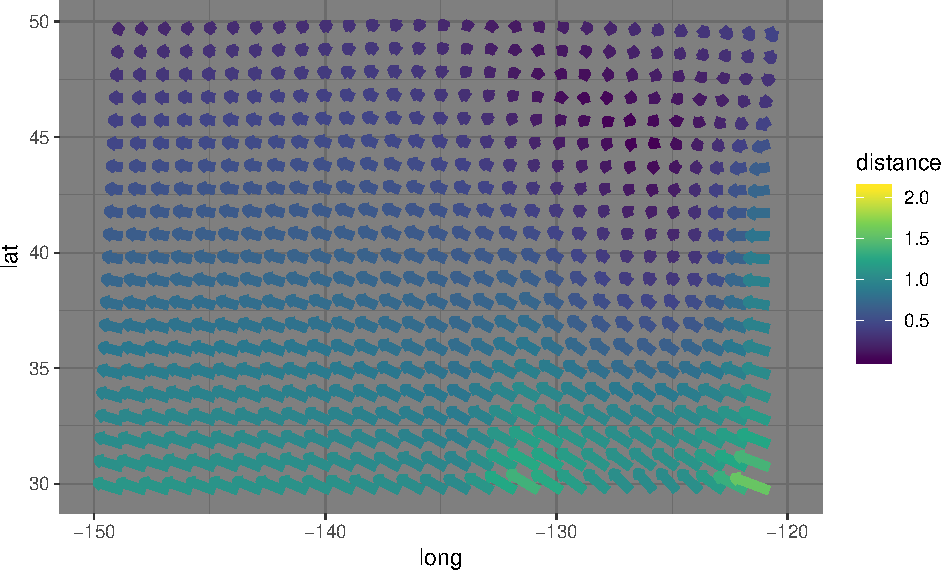
\includegraphics{R_tidyverse_for_geographers_files/figure-latex/unnamed-chunk-24-1.pdf}

\begin{Shaded}
\begin{Highlighting}[]
\KeywordTok{plot}\NormalTok{(}\KeywordTok{density}\NormalTok{(carb}\OperatorTok{$}\NormalTok{height_cm)) }\CommentTok{# base-R way to plot kernel density}
\end{Highlighting}
\end{Shaded}

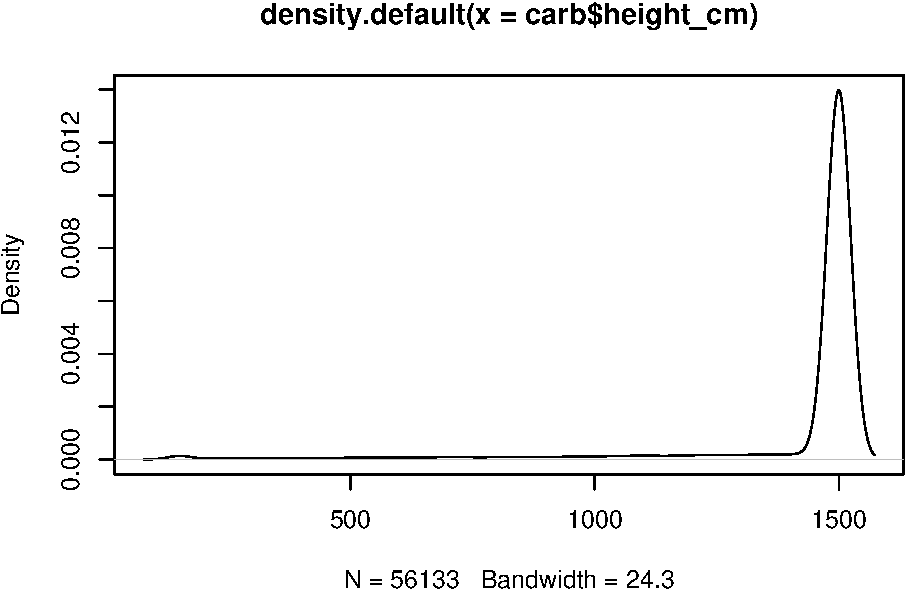
\includegraphics{R_tidyverse_for_geographers_files/figure-latex/unnamed-chunk-24-2.pdf}

\begin{Shaded}
\begin{Highlighting}[]
\NormalTok{carb }\OperatorTok\StringTok{ }\NormalTok{glimpse}
\end{Highlighting}
\end{Shaded}

\begin{verbatim}
## Observations: 56,133
## Variables: 7
## $ year      <int> 1999, 1999, 1999, 1999, 1999, 1999, 1999, 1999, 1999...
## $ plot      <chr> "A1", "A1", "A1", "A1", "A1", "A1", "A1", "A1", "A1"...
## $ Y_m       <int> 15, 20, 30, 20, 0, 35, 30, 20, 25, 30, 30, 40, 25, 2...
## $ X_m       <int> 85, 10, 0, 100, 95, 45, 45, 65, 45, 100, 50, 15, 10,...
## $ height_cm <int> 150, 150, 150, 507, 579, 695, 712, 788, 811, 835, 83...
## $ Comments  <chr> "Not done in 1999", "Not done in 1999", "Not done in...
## $ date      <dttm> 1999-07-12, 1999-07-12, 1999-07-12, 1999-07-12, 199...
\end{verbatim}

\begin{Shaded}
\begin{Highlighting}[]
\NormalTok{carb }\OperatorTok\StringTok{ }\KeywordTok{ggplot}\NormalTok{(}\DataTypeTok{data=}\NormalTok{., }\KeywordTok{aes}\NormalTok{(}\DataTypeTok{x=}\NormalTok{height_cm))}\OperatorTok{+}\KeywordTok{geom_histogram}\NormalTok{()}
\end{Highlighting}
\end{Shaded}

\begin{verbatim}
## `stat_bin()` using `bins = 30`. Pick better value with `binwidth`.
\end{verbatim}

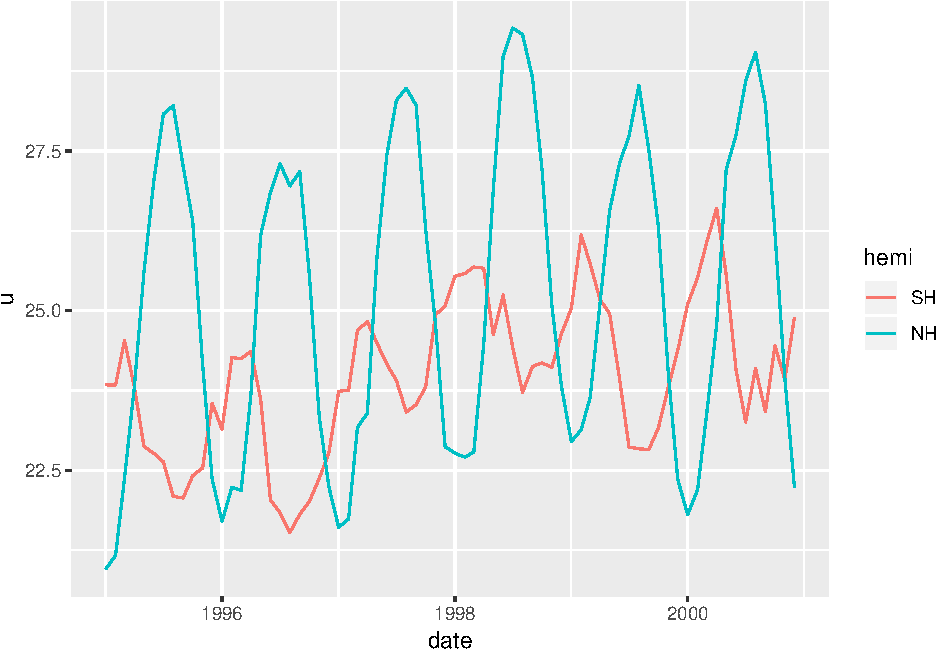
\includegraphics{R_tidyverse_for_geographers_files/figure-latex/unnamed-chunk-24-3.pdf}

\begin{Shaded}
\begin{Highlighting}[]
\NormalTok{carb }\OperatorTok\StringTok{ }
\StringTok{  }\KeywordTok{filter}\NormalTok{(}\KeywordTok{near}\NormalTok{(year,}\DecValTok{2000}\NormalTok{,}\DataTypeTok{tol =} \FloatTok{0.1}\NormalTok{)) }\OperatorTok\StringTok{ }\CommentTok{# filtering for numbers can be tricky, use near to specify a filter with a tolerance}
\StringTok{  }\KeywordTok{ggplot}\NormalTok{(}\DataTypeTok{data=}\NormalTok{., }\KeywordTok{aes}\NormalTok{(}\DataTypeTok{x=}\NormalTok{height_cm))}\OperatorTok{+}\KeywordTok{geom_histogram}\NormalTok{()}\OperatorTok{+}\KeywordTok{facet_wrap}\NormalTok{(}\OperatorTok{~}\NormalTok{plot)}
\end{Highlighting}
\end{Shaded}

\begin{verbatim}
## `stat_bin()` using `bins = 30`. Pick better value with `binwidth`.
\end{verbatim}

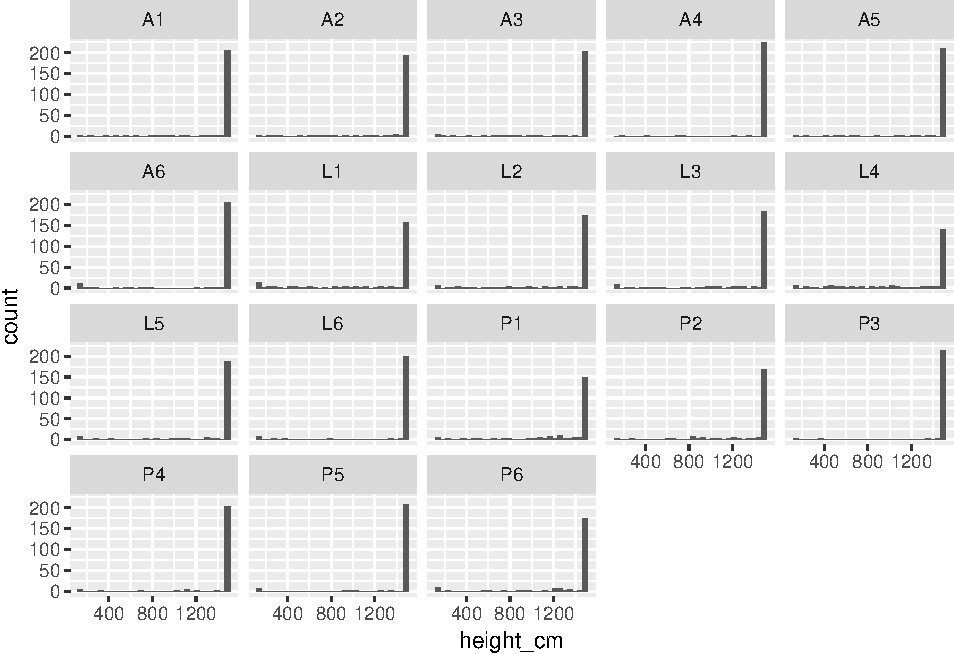
\includegraphics{R_tidyverse_for_geographers_files/figure-latex/unnamed-chunk-24-4.pdf}

\begin{Shaded}
\begin{Highlighting}[]
\NormalTok{carb }\OperatorTok\StringTok{ }
\StringTok{  }\KeywordTok{filter}\NormalTok{(}\KeywordTok{near}\NormalTok{(year,}\DecValTok{2000}\NormalTok{,}\DataTypeTok{tol =} \FloatTok{0.1}\NormalTok{)) }\OperatorTok\StringTok{ }
\StringTok{  }\KeywordTok{ggplot}\NormalTok{(}\DataTypeTok{data=}\NormalTok{., }\KeywordTok{aes}\NormalTok{(}\DataTypeTok{x=} \KeywordTok{log1p}\NormalTok{(height_cm)))}\OperatorTok{+}
\StringTok{  }\KeywordTok{geom_histogram}\NormalTok{(}\DataTypeTok{bins =} \DecValTok{10}\NormalTok{)}\OperatorTok{+}
\StringTok{  }\KeywordTok{scale_y_continuous}\NormalTok{(}\DataTypeTok{trans=}\StringTok{"log1p"}\NormalTok{)}\OperatorTok{+}
\StringTok{  }\KeywordTok{facet_wrap}\NormalTok{(}\OperatorTok{~}\NormalTok{plot)}
\end{Highlighting}
\end{Shaded}

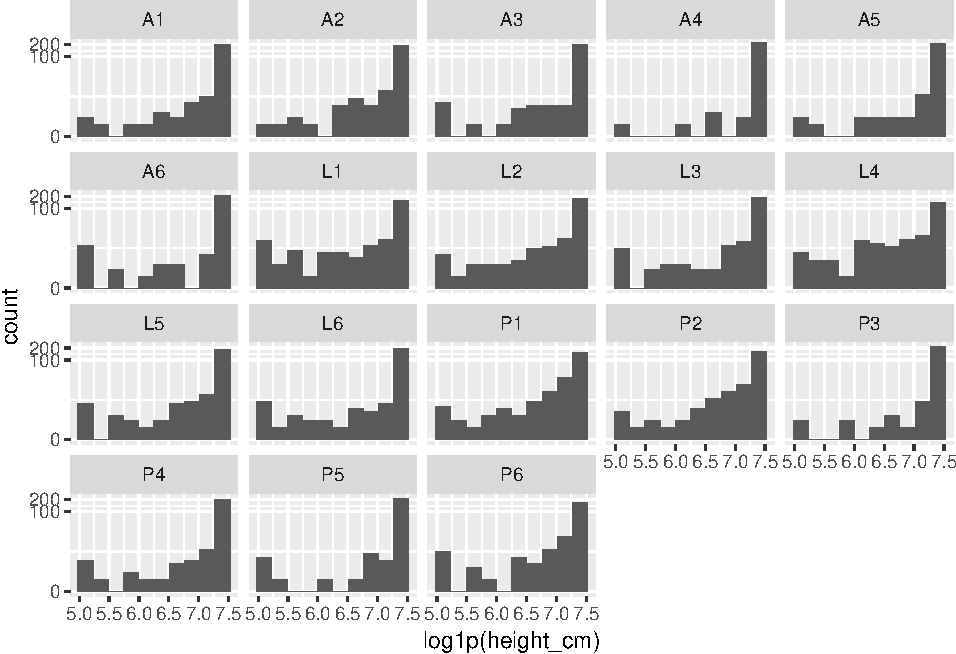
\includegraphics{R_tidyverse_for_geographers_files/figure-latex/unnamed-chunk-24-5.pdf}
\# Spatiotemporal example
--------------------------------------------------

\begin{Shaded}
\begin{Highlighting}[]
\NormalTok{nasa}
\end{Highlighting}
\end{Shaded}

\begin{verbatim}
## Source: local array [41,472 x 4]
## D: lat [dbl, 24]
## D: long [dbl, 24]
## D: month [int, 12]
## D: year [int, 6]
## M: cloudhigh [dbl]
## M: cloudlow [dbl]
## M: cloudmid [dbl]
## M: ozone [dbl]
## M: pressure [dbl]
## M: surftemp [dbl]
## M: temperature [dbl]
\end{verbatim}

\begin{Shaded}
\begin{Highlighting}[]
\NormalTok{nasa }\OperatorTok\StringTok{ }\KeywordTok{glimpse}\NormalTok{()}
\end{Highlighting}
\end{Shaded}

\begin{verbatim}
## List of 2
##  $ mets:List of 7
##   ..$ cloudhigh  : num [1:24, 1:24, 1:12, 1:6] 26 20 16 13 7.5 8 14.5 19.5 22.5 21 ...
##   ..$ cloudlow   : num [1:24, 1:24, 1:12, 1:6] 7.5 11.5 16.5 20.5 26 30 29.5 26.5 27.5 26 ...
##   ..$ cloudmid   : num [1:24, 1:24, 1:12, 1:6] 34.5 32.5 26 14.5 10.5 9.5 11 17.5 18.5 16.5 ...
##   ..$ ozone      : num [1:24, 1:24, 1:12, 1:6] 304 304 298 276 274 264 258 252 250 250 ...
##   ..$ pressure   : num [1:24, 1:24, 1:12, 1:6] 835 940 960 990 1000 1000 1000 1000 1000 1000 ...
##   ..$ surftemp   : num [1:24, 1:24, 1:12, 1:6] 273 280 285 289 292 ...
##   ..$ temperature: num [1:24, 1:24, 1:12, 1:6] 272 282 285 291 293 ...
##  $ dims:List of 4
##   ..$ lat  : num [1:24] 36.2 33.7 31.2 28.7 26.2 ...
##   ..$ long : num [1:24] -114 -111 -109 -106 -104 ...
##   ..$ month: int [1:12] 1 2 3 4 5 6 7 8 9 10 ...
##   ..$ year : int [1:6] 1995 1996 1997 1998 1999 2000
##  - attr(*, "class")= chr "tbl_cube"
\end{verbatim}

\begin{Shaded}
\begin{Highlighting}[]
\NormalTok{nasa }\OperatorTok\StringTok{ }
\StringTok{  }\KeywordTok{as_tibble}\NormalTok{() }\OperatorTok\StringTok{ }
\StringTok{  }\KeywordTok{ggplot}\NormalTok{(}\DataTypeTok{data=}\NormalTok{., }\KeywordTok{aes}\NormalTok{(long,lat))}\OperatorTok{+}
\StringTok{  }\KeywordTok{geom_raster}\NormalTok{(}\KeywordTok{aes}\NormalTok{(}\DataTypeTok{fill=}\NormalTok{ozone))}\OperatorTok{+}
\StringTok{  }\KeywordTok{coord_equal}\NormalTok{()}\OperatorTok{+}
\StringTok{  }\KeywordTok{scale_fill_viridis_c}\NormalTok{() }\OperatorTok{+}\StringTok{ }
\StringTok{  }\KeywordTok{facet_wrap}\NormalTok{(}\OperatorTok{~}\NormalTok{month)}
\end{Highlighting}
\end{Shaded}

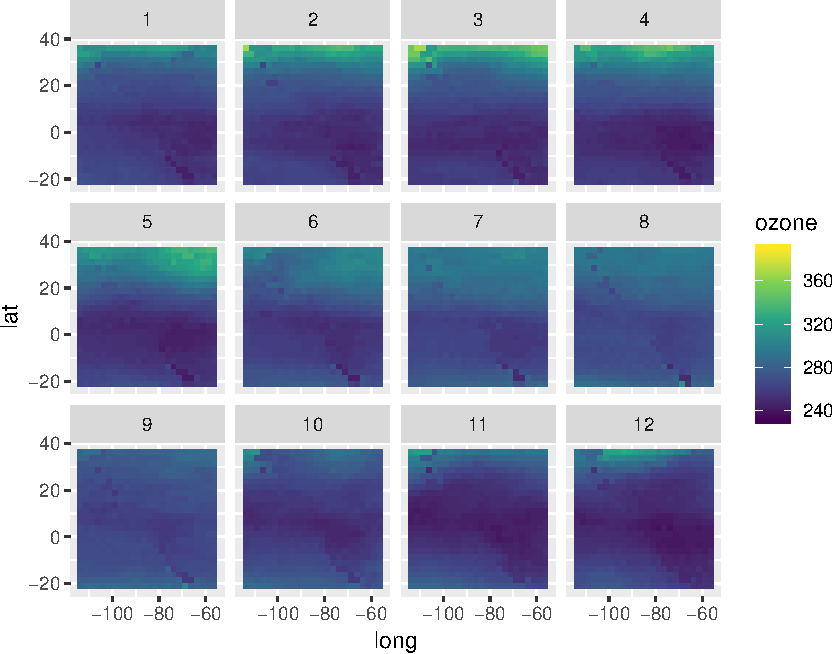
\includegraphics{R_tidyverse_for_geographers_files/figure-latex/unnamed-chunk-26-1.pdf}

\begin{Shaded}
\begin{Highlighting}[]
\NormalTok{nasa }\OperatorTok\StringTok{ }
\StringTok{  }\KeywordTok{as_tibble}\NormalTok{() }\OperatorTok\StringTok{ }
\StringTok{  }\KeywordTok{group_by}\NormalTok{(lat,long, month) }\OperatorTok\StringTok{ }
\StringTok{  }\KeywordTok{summarize}\NormalTok{(}\DataTypeTok{u=}\KeywordTok{mean}\NormalTok{(temperature,}\DataTypeTok{na.rm=}\NormalTok{T)) }\OperatorTok\StringTok{ }
\StringTok{  }\KeywordTok{ggplot}\NormalTok{(}\DataTypeTok{data=}\NormalTok{., }\KeywordTok{aes}\NormalTok{(long,lat))}\OperatorTok{+}
\StringTok{  }\KeywordTok{geom_raster}\NormalTok{(}\KeywordTok{aes}\NormalTok{(}\DataTypeTok{fill=}\NormalTok{u))}\OperatorTok{+}
\StringTok{  }\KeywordTok{coord_equal}\NormalTok{()}\OperatorTok{+}
\StringTok{  }\KeywordTok{scale_fill_viridis_c}\NormalTok{() }\OperatorTok{+}\StringTok{ }
\StringTok{  }\KeywordTok{facet_wrap}\NormalTok{(}\OperatorTok{~}\NormalTok{month)}
\end{Highlighting}
\end{Shaded}

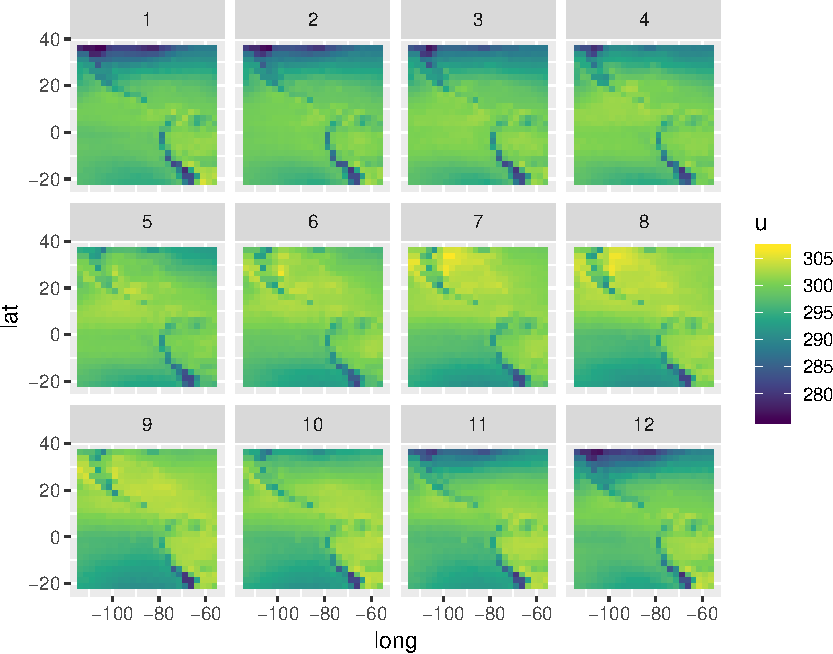
\includegraphics{R_tidyverse_for_geographers_files/figure-latex/unnamed-chunk-27-1.pdf}

\begin{Shaded}
\begin{Highlighting}[]
\NormalTok{nasa }\OperatorTok\StringTok{ }
\StringTok{  }\KeywordTok{as_tibble}\NormalTok{() }\OperatorTok\StringTok{ }
\StringTok{  }\KeywordTok{group_by}\NormalTok{(lat,long, month) }\OperatorTok\StringTok{ }
\StringTok{  }\KeywordTok{summarize}\NormalTok{(}\DataTypeTok{u=}\KeywordTok{mean}\NormalTok{(temperature,}\DataTypeTok{na.rm=}\NormalTok{T)) }\OperatorTok\StringTok{ }
\StringTok{  }\KeywordTok{ungroup}\NormalTok{() }\OperatorTok\StringTok{ }
\StringTok{  }\KeywordTok{mutate}\NormalTok{(}\DataTypeTok{tempC =}\NormalTok{ u }\OperatorTok{-}\StringTok{ }\FloatTok{273.15}\NormalTok{) }\OperatorTok\StringTok{ }
\StringTok{  }\KeywordTok{ggplot}\NormalTok{(}\DataTypeTok{data=}\NormalTok{., }\KeywordTok{aes}\NormalTok{(long,lat))}\OperatorTok{+}
\StringTok{  }\KeywordTok{geom_raster}\NormalTok{(}\KeywordTok{aes}\NormalTok{(}\DataTypeTok{fill=}\NormalTok{tempC))}\OperatorTok{+}
\StringTok{  }\KeywordTok{coord_equal}\NormalTok{()}\OperatorTok{+}
\StringTok{  }\KeywordTok{scale_fill_viridis_c}\NormalTok{() }\OperatorTok{+}\StringTok{ }
\StringTok{  }\KeywordTok{facet_wrap}\NormalTok{(}\OperatorTok{~}\NormalTok{month)}
\end{Highlighting}
\end{Shaded}

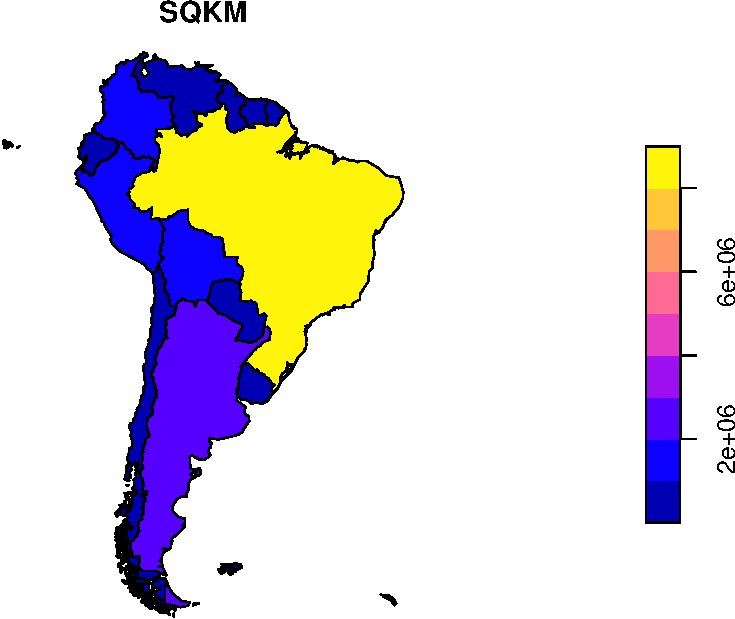
\includegraphics{R_tidyverse_for_geographers_files/figure-latex/unnamed-chunk-27-2.pdf}

\begin{Shaded}
\begin{Highlighting}[]
\NormalTok{nasa }\OperatorTok\StringTok{ }
\StringTok{  }\KeywordTok{as_tibble}\NormalTok{() }\OperatorTok\StringTok{ }
\StringTok{  }\KeywordTok{group_by}\NormalTok{(lat,long, year,month) }\OperatorTok\StringTok{ }
\StringTok{  }\CommentTok{# summarize(u=mean(temperature,na.rm=T)) %>% }
\StringTok{  }\CommentTok{# ungroup() %>% }
\StringTok{  }\KeywordTok{mutate}\NormalTok{(}\DataTypeTok{tempC =}\NormalTok{ temperature }\OperatorTok{-}\StringTok{ }\FloatTok{273.15}\NormalTok{) }\OperatorTok\StringTok{ }
\StringTok{  }\KeywordTok{mutate}\NormalTok{(}\DataTypeTok{hemi =} \KeywordTok{cut}\NormalTok{(lat,}\DataTypeTok{breaks =} \KeywordTok{c}\NormalTok{(}\OperatorTok{-}\OtherTok{Inf}\NormalTok{,}\DecValTok{0}\NormalTok{,}\OtherTok{Inf}\NormalTok{),}\DataTypeTok{labels =} \KeywordTok{c}\NormalTok{(}\StringTok{"SH"}\NormalTok{,}\StringTok{"NH"}\NormalTok{))) }\OperatorTok\StringTok{ }
\StringTok{  }\KeywordTok{group_by}\NormalTok{(hemi,year,month) }\OperatorTok\StringTok{ }
\StringTok{  }\KeywordTok{summarize}\NormalTok{(}\DataTypeTok{u=}\KeywordTok{mean}\NormalTok{(tempC,}\DataTypeTok{na.rm=}\NormalTok{T)) }\OperatorTok\StringTok{ }
\StringTok{  }\KeywordTok{ungroup}\NormalTok{() }\OperatorTok\StringTok{ }
\StringTok{  }\KeywordTok{mutate}\NormalTok{(}\DataTypeTok{date=}\KeywordTok{parse_date_time}\NormalTok{(}\KeywordTok{paste}\NormalTok{(year,month,}\DecValTok{1}\NormalTok{),}\StringTok{'ymd'}\NormalTok{)) }\OperatorTok\StringTok{ }
\StringTok{  }\KeywordTok{ggplot}\NormalTok{(}\DataTypeTok{data=}\NormalTok{., }\KeywordTok{aes}\NormalTok{(date,u,}\DataTypeTok{color=}\NormalTok{hemi))}\OperatorTok{+}
\StringTok{  }\KeywordTok{geom_line}\NormalTok{()}\OperatorTok{+}
\StringTok{  }\KeywordTok{scale_fill_viridis_c}\NormalTok{() }
\end{Highlighting}
\end{Shaded}

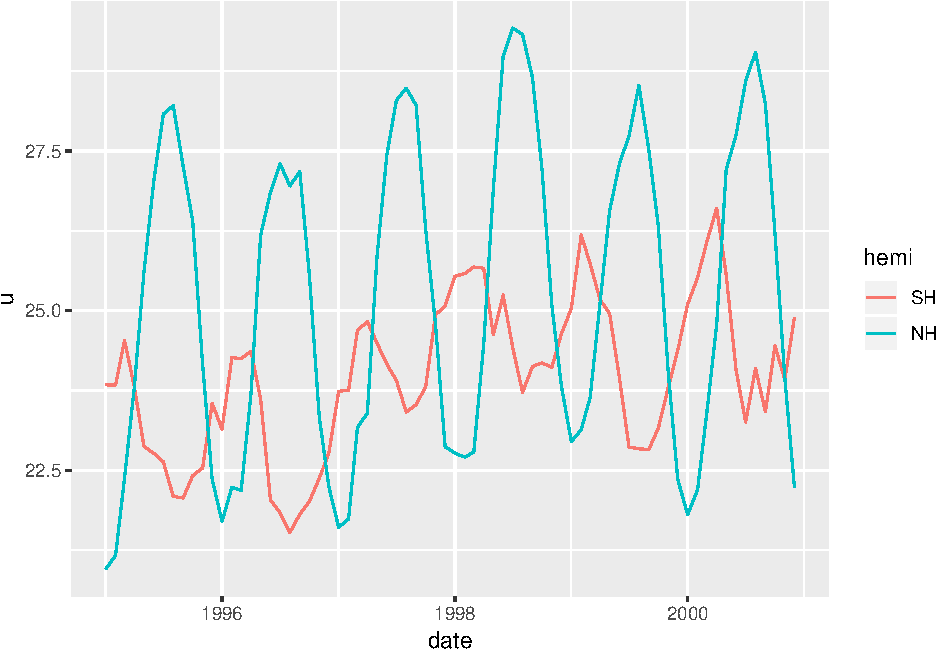
\includegraphics{R_tidyverse_for_geographers_files/figure-latex/unnamed-chunk-27-3.pdf}

\hypertarget{seals--}{%
\section{Seals
-------------------------------------------------------------------}\label{seals--}}

\begin{Shaded}
\begin{Highlighting}[]
\KeywordTok{data}\NormalTok{(}\StringTok{"seals"}\NormalTok{)}
\NormalTok{seals }\OperatorTok\StringTok{ }\NormalTok{glimpse}
\end{Highlighting}
\end{Shaded}

\begin{verbatim}
## Observations: 1,155
## Variables: 4
## $ lat        <dbl> 29.7, 30.7, 31.7, 32.7, 33.7, 34.7, 35.7, 36.7, 37....
## $ long       <dbl> -172.8, -172.8, -172.8, -172.8, -172.8, -172.8, -17...
## $ delta_long <dbl> -0.91504624, -0.86701252, -0.81892489, -0.77077630,...
## $ delta_lat  <dbl> 0.143475254, 0.128388724, 0.113232481, 0.098020371,...
\end{verbatim}

\begin{Shaded}
\begin{Highlighting}[]
\NormalTok{seals }\OperatorTok\StringTok{ }
\StringTok{  }\KeywordTok{mutate}\NormalTok{(}\DataTypeTok{distance=}\KeywordTok{sqrt}\NormalTok{(delta_long}\OperatorTok{**}\DecValTok{2} \OperatorTok{+}\StringTok{ }\NormalTok{delta_lat}\OperatorTok{**}\DecValTok{2}\NormalTok{)) }\OperatorTok\StringTok{ }
\StringTok{  }\KeywordTok{ggplot}\NormalTok{(., }\KeywordTok{aes}\NormalTok{(long, lat, }\DataTypeTok{color=}\NormalTok{distance)) }\OperatorTok{+}
\StringTok{  }\KeywordTok{geom_segment}\NormalTok{(}\KeywordTok{aes}\NormalTok{(}\DataTypeTok{xend =}\NormalTok{ long }\OperatorTok{+}\StringTok{ }\NormalTok{delta_long, }\DataTypeTok{yend =}\NormalTok{ lat }\OperatorTok{+}\StringTok{ }\NormalTok{delta_lat),}
               \DataTypeTok{arrow =} \KeywordTok{arrow}\NormalTok{(}\DataTypeTok{length =} \KeywordTok{unit}\NormalTok{(}\FloatTok{0.1}\NormalTok{,}\StringTok{"cm"}\NormalTok{)),}\DataTypeTok{lwd=}\DecValTok{2}\NormalTok{) }\OperatorTok{+}
\StringTok{  }\KeywordTok{coord_equal}\NormalTok{()}\OperatorTok{+}
\StringTok{  }\KeywordTok{borders}\NormalTok{(}\StringTok{"usa"}\NormalTok{)}\OperatorTok{+}
\StringTok{  }\KeywordTok{scale_x_continuous}\NormalTok{(}\DataTypeTok{limits =} \KeywordTok{c}\NormalTok{(}\OperatorTok{-}\DecValTok{150}\NormalTok{,}\OperatorTok{-}\DecValTok{120}\NormalTok{))}\OperatorTok{+}
\StringTok{  }\KeywordTok{scale_color_viridis_c}\NormalTok{()}\OperatorTok{+}
\StringTok{  }\KeywordTok{theme_dark}\NormalTok{()}
\end{Highlighting}
\end{Shaded}

\begin{verbatim}
## 
## Attaching package: 'maps'
\end{verbatim}

\begin{verbatim}
## The following object is masked from 'package:purrr':
## 
##     map
\end{verbatim}

\begin{verbatim}
## Warning: Removed 546 rows containing missing values (geom_segment).
\end{verbatim}

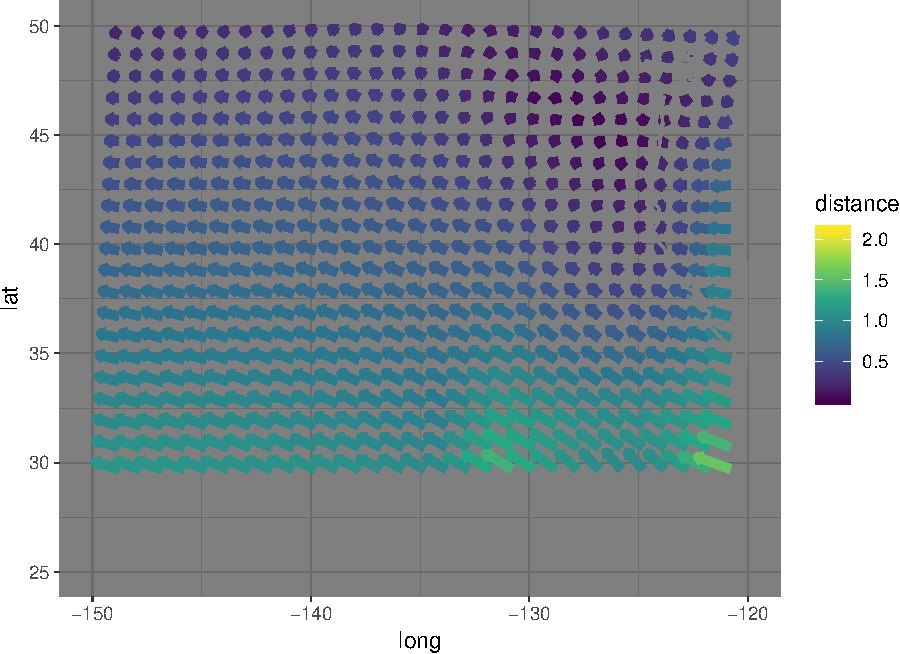
\includegraphics{R_tidyverse_for_geographers_files/figure-latex/unnamed-chunk-28-1.pdf}

\hypertarget{storms}{%
\section{storms
------------------------------------------------------------------}\label{storms}}

\begin{Shaded}
\begin{Highlighting}[]
\KeywordTok{library}\NormalTok{(tidyverse)}
\NormalTok{dplyr}\OperatorTok{::}\NormalTok{storms}
\end{Highlighting}
\end{Shaded}

\begin{verbatim}
## # A tibble: 10,010 x 13
##    name   year month   day  hour   lat  long status         category  wind
##    <chr> <dbl> <dbl> <int> <dbl> <dbl> <dbl> <chr>          <ord>    <int>
##  1 Amy    1975     6    27     0  27.5 -79   tropical depr~ -1          25
##  2 Amy    1975     6    27     6  28.5 -79   tropical depr~ -1          25
##  3 Amy    1975     6    27    12  29.5 -79   tropical depr~ -1          25
##  4 Amy    1975     6    27    18  30.5 -79   tropical depr~ -1          25
##  5 Amy    1975     6    28     0  31.5 -78.8 tropical depr~ -1          25
##  6 Amy    1975     6    28     6  32.4 -78.7 tropical depr~ -1          25
##  7 Amy    1975     6    28    12  33.3 -78   tropical depr~ -1          25
##  8 Amy    1975     6    28    18  34   -77   tropical depr~ -1          30
##  9 Amy    1975     6    29     0  34.4 -75.8 tropical storm 0           35
## 10 Amy    1975     6    29     6  34   -74.8 tropical storm 0           40
## # ... with 10,000 more rows, and 3 more variables: pressure <int>,
## #   ts_diameter <dbl>, hu_diameter <dbl>
\end{verbatim}

\begin{Shaded}
\begin{Highlighting}[]
\KeywordTok{names}\NormalTok{(storms)}
\end{Highlighting}
\end{Shaded}

\begin{verbatim}
##  [1] "name"        "year"        "month"       "day"         "hour"       
##  [6] "lat"         "long"        "status"      "category"    "wind"       
## [11] "pressure"    "ts_diameter" "hu_diameter"
\end{verbatim}

\begin{Shaded}
\begin{Highlighting}[]
\CommentTok{# bad!}
\NormalTok{storms }\OperatorTok
\StringTok{  }\KeywordTok{ggplot}\NormalTok{(}\DataTypeTok{data=}\NormalTok{., }\KeywordTok{aes}\NormalTok{(long,lat,}\DataTypeTok{size=}\NormalTok{category))}\OperatorTok{+}
\StringTok{  }\KeywordTok{geom_point}\NormalTok{()}\OperatorTok{+}
\StringTok{  }\CommentTok{# borders("world")+}
\StringTok{  }\KeywordTok{scale_x_continuous}\NormalTok{(}\DataTypeTok{limits=}\KeywordTok{c}\NormalTok{(}\OperatorTok{-}\DecValTok{120}\NormalTok{,}\DecValTok{0}\NormalTok{))}\OperatorTok{+}
\StringTok{  }\KeywordTok{scale_y_continuous}\NormalTok{(}\DataTypeTok{limits =} \KeywordTok{c}\NormalTok{(}\OperatorTok{-}\DecValTok{10}\NormalTok{,}\DecValTok{55}\NormalTok{))}\OperatorTok{+}
\StringTok{  }\KeywordTok{borders}\NormalTok{(}\StringTok{'world'}\NormalTok{, }\DataTypeTok{fill =} \StringTok{"brown"}\NormalTok{)}
\end{Highlighting}
\end{Shaded}

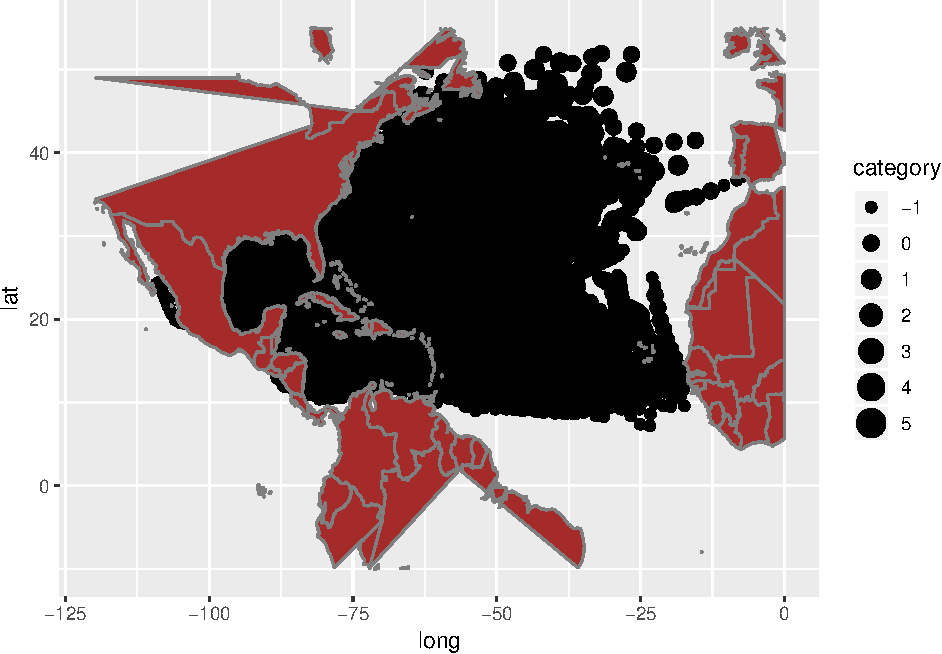
\includegraphics{R_tidyverse_for_geographers_files/figure-latex/dplyr::storms-1.pdf}

\begin{Shaded}
\begin{Highlighting}[]
\CommentTok{# bad!}
\NormalTok{storms }\OperatorTok\StringTok{ }
\StringTok{  }\KeywordTok{arrange}\NormalTok{(wind) }\OperatorTok\StringTok{ }
\StringTok{  }\KeywordTok{ggplot}\NormalTok{(}\DataTypeTok{data=}\NormalTok{., }\KeywordTok{aes}\NormalTok{(long,lat,}\DataTypeTok{size=}\NormalTok{category,}\DataTypeTok{color=}\NormalTok{wind))}\OperatorTok{+}
\StringTok{  }\CommentTok{# borders("coast")+}
\StringTok{  }\KeywordTok{geom_point}\NormalTok{()}\OperatorTok{+}
\StringTok{  }\KeywordTok{scale_color_viridis_c}\NormalTok{()}\OperatorTok{+}
\StringTok{  }\KeywordTok{scale_x_continuous}\NormalTok{(}\DataTypeTok{limits=}\KeywordTok{c}\NormalTok{(}\OperatorTok{-}\DecValTok{130}\NormalTok{,}\DecValTok{0}\NormalTok{))}\OperatorTok{+}
\StringTok{  }\KeywordTok{scale_y_continuous}\NormalTok{(}\DataTypeTok{limits =} \KeywordTok{c}\NormalTok{(}\OperatorTok{-}\DecValTok{10}\NormalTok{,}\DecValTok{55}\NormalTok{))}
\end{Highlighting}
\end{Shaded}

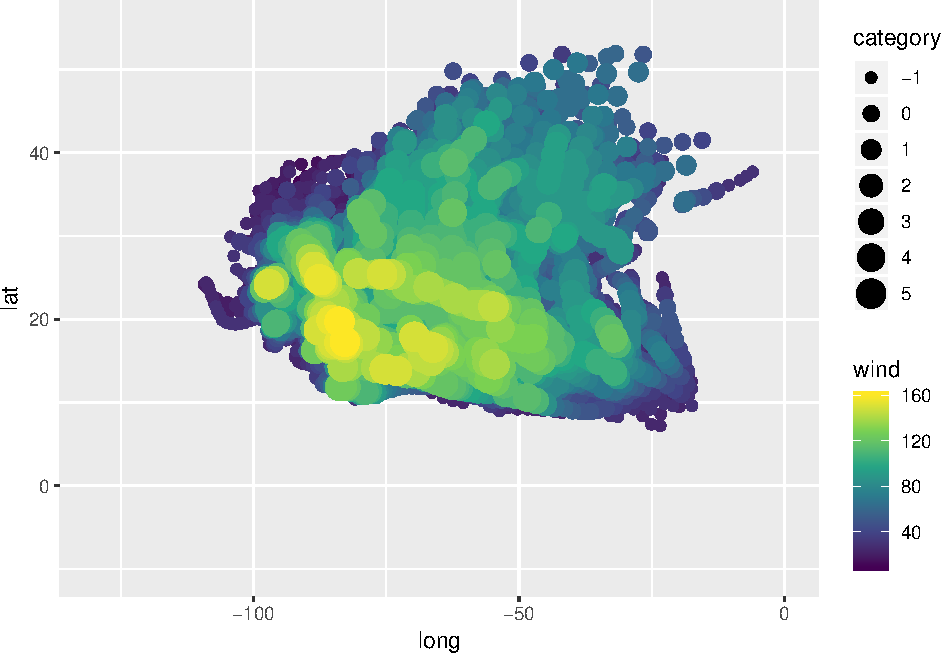
\includegraphics{R_tidyverse_for_geographers_files/figure-latex/dplyr::storms-2.pdf}

\begin{Shaded}
\begin{Highlighting}[]
\NormalTok{storms }\OperatorTok\StringTok{ }\KeywordTok{group_by}\NormalTok{(year) }\OperatorTok\StringTok{ }\KeywordTok{summarize}\NormalTok{(}\DataTypeTok{nobs=}\KeywordTok{n}\NormalTok{()) }\OperatorTok\StringTok{ }\KeywordTok{ggplot}\NormalTok{(}\DataTypeTok{data=}\NormalTok{., }\KeywordTok{aes}\NormalTok{(year,nobs))}\OperatorTok{+}\KeywordTok{geom_line}\NormalTok{()}
\end{Highlighting}
\end{Shaded}

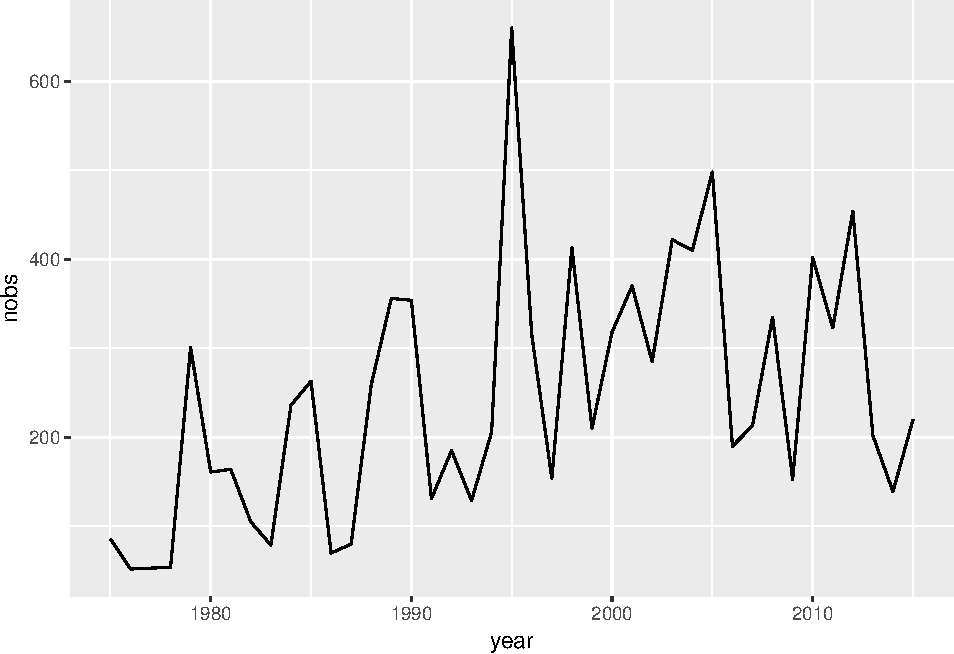
\includegraphics{R_tidyverse_for_geographers_files/figure-latex/dplyr::storms-3.pdf}

\begin{Shaded}
\begin{Highlighting}[]
\NormalTok{storms }\OperatorTok\StringTok{ }\KeywordTok{group_by}\NormalTok{(month) }\OperatorTok\StringTok{ }\KeywordTok{summarize}\NormalTok{(}\DataTypeTok{wind_25=}\KeywordTok{quantile}\NormalTok{(wind,}\FloatTok{0.025}\NormalTok{), }
                                         \DataTypeTok{wind_50=}\KeywordTok{median}\NormalTok{(wind), }
                                         \DataTypeTok{wind_75=}\KeywordTok{quantile}\NormalTok{(wind, }\FloatTok{0.95}\NormalTok{)) }\OperatorTok\StringTok{ }
\StringTok{  }\KeywordTok{ungroup}\NormalTok{() }\OperatorTok\StringTok{ }
\StringTok{  }\KeywordTok{ggplot}\NormalTok{(}\DataTypeTok{data=}\NormalTok{., }\KeywordTok{aes}\NormalTok{(month, wind_}\DecValTok{50}\NormalTok{))}\OperatorTok{+}
\StringTok{  }\KeywordTok{geom_ribbon}\NormalTok{(}\KeywordTok{aes}\NormalTok{(}\DataTypeTok{x=}\NormalTok{month, }\DataTypeTok{ymax=}\NormalTok{wind_}\DecValTok{75}\NormalTok{, }\DataTypeTok{ymin=}\NormalTok{wind_}\DecValTok{25}\NormalTok{),}\DataTypeTok{lty=}\DecValTok{0}\NormalTok{,}\DataTypeTok{alpha=}\FloatTok{0.25}\NormalTok{)}\OperatorTok{+}
\StringTok{  }\KeywordTok{geom_line}\NormalTok{()}\OperatorTok{+}
\StringTok{  }\KeywordTok{labs}\NormalTok{(}\DataTypeTok{x=}\StringTok{"Month"}\NormalTok{,}\DataTypeTok{y=}\StringTok{"Wind speed [knots]"}\NormalTok{,}\DataTypeTok{title =} \StringTok{"95% quantile rate of hurricane wind speed"}\NormalTok{)}
\end{Highlighting}
\end{Shaded}

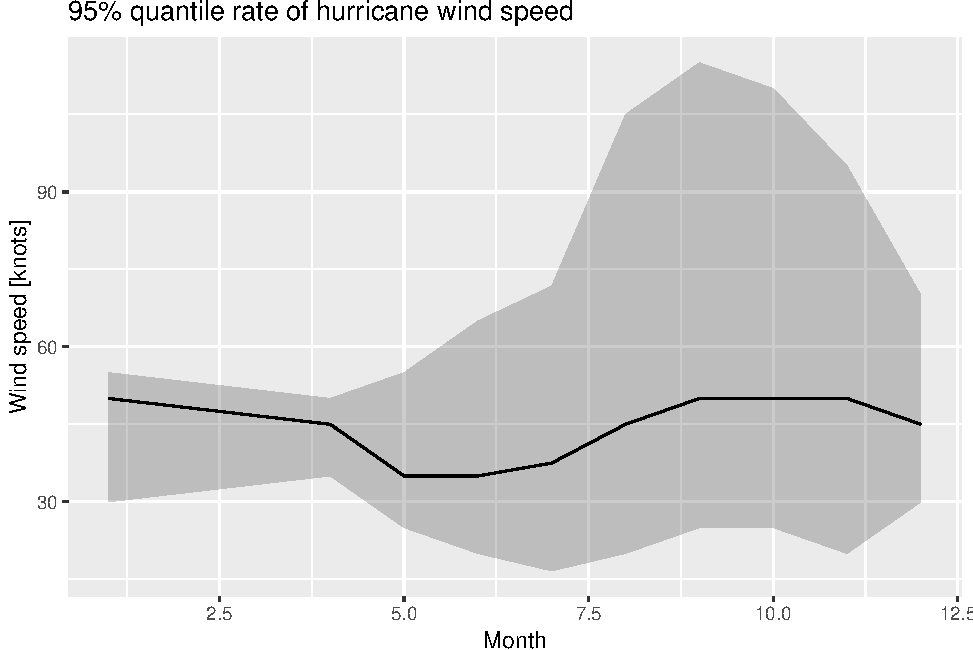
\includegraphics{R_tidyverse_for_geographers_files/figure-latex/dplyr::storms-4.pdf}

\begin{Shaded}
\begin{Highlighting}[]
\CommentTok{# swap 'month' for 'year'}
\NormalTok{storms }\OperatorTok\StringTok{ }\KeywordTok{group_by}\NormalTok{(year) }\OperatorTok\StringTok{ }\KeywordTok{summarize}\NormalTok{(}\DataTypeTok{wind_25=}\KeywordTok{quantile}\NormalTok{(wind,}\FloatTok{0.025}\NormalTok{), }
                                         \DataTypeTok{wind_50=}\KeywordTok{median}\NormalTok{(wind), }
                                         \DataTypeTok{wind_75=}\KeywordTok{quantile}\NormalTok{(wind, }\FloatTok{0.95}\NormalTok{)) }\OperatorTok\StringTok{ }
\StringTok{  }\KeywordTok{ungroup}\NormalTok{() }\OperatorTok\StringTok{ }
\StringTok{  }\KeywordTok{ggplot}\NormalTok{(}\DataTypeTok{data=}\NormalTok{., }\KeywordTok{aes}\NormalTok{(year, wind_}\DecValTok{50}\NormalTok{))}\OperatorTok{+}
\StringTok{  }\KeywordTok{geom_ribbon}\NormalTok{(}\KeywordTok{aes}\NormalTok{(}\DataTypeTok{x=}\NormalTok{year, }\DataTypeTok{ymax=}\NormalTok{wind_}\DecValTok{75}\NormalTok{, }\DataTypeTok{ymin=}\NormalTok{wind_}\DecValTok{25}\NormalTok{),}\DataTypeTok{lty=}\DecValTok{0}\NormalTok{,}\DataTypeTok{alpha=}\FloatTok{0.25}\NormalTok{)}\OperatorTok{+}
\StringTok{  }\KeywordTok{geom_line}\NormalTok{()}\OperatorTok{+}
\StringTok{  }\KeywordTok{labs}\NormalTok{(}\DataTypeTok{x=}\StringTok{"Month"}\NormalTok{,}\DataTypeTok{y=}\StringTok{"Wind speed [knots]"}\NormalTok{,}\DataTypeTok{title =} \StringTok{"95% quantile rate of hurricane wind speed"}\NormalTok{)}
\end{Highlighting}
\end{Shaded}

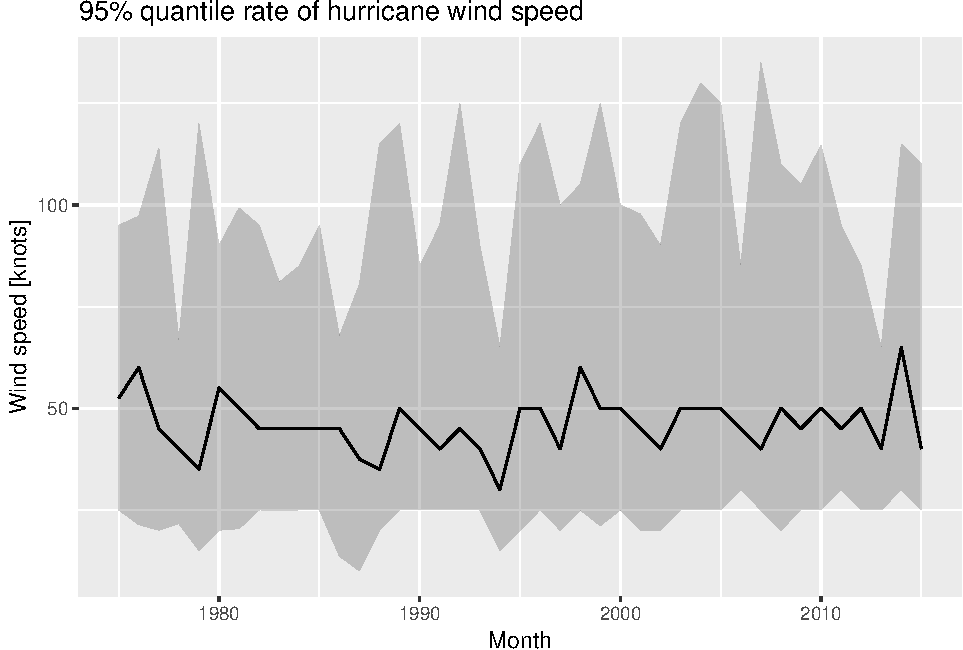
\includegraphics{R_tidyverse_for_geographers_files/figure-latex/dplyr::storms-5.pdf}

\begin{Shaded}
\begin{Highlighting}[]
\CommentTok{# advanced!}
\NormalTok{p =}\StringTok{ }\KeywordTok{c}\NormalTok{(}\FloatTok{0.025}\NormalTok{, }\FloatTok{0.25}\NormalTok{,}\FloatTok{0.5}\NormalTok{,}\FloatTok{0.75}\NormalTok{,}\FloatTok{0.975}\NormalTok{)}
\NormalTok{storms }\OperatorTok\StringTok{ }
\StringTok{  }\KeywordTok{group_by}\NormalTok{(month) }\OperatorTok\StringTok{ }
\StringTok{  }\KeywordTok{summarise}\NormalTok{(}\DataTypeTok{quantiles =} \KeywordTok{list}\NormalTok{(}\KeywordTok{sprintf}\NormalTok{(}\StringTok{"%1.0f%%"}\NormalTok{, p}\OperatorTok{*}\DecValTok{100}\NormalTok{)),}
            \DataTypeTok{wind =} \KeywordTok{list}\NormalTok{(}\KeywordTok{quantile}\NormalTok{(wind, p))) }\OperatorTok\StringTok{ }
\StringTok{  }\NormalTok{unnest }\OperatorTok\StringTok{ }
\StringTok{  }\KeywordTok{ggplot}\NormalTok{(}\DataTypeTok{data=}\NormalTok{., }\KeywordTok{aes}\NormalTok{(month, wind, }\DataTypeTok{color=}\NormalTok{quantiles))}\OperatorTok{+}
\StringTok{  }\KeywordTok{geom_line}\NormalTok{()}\OperatorTok{+}
\StringTok{  }\KeywordTok{scale_color_viridis_d}\NormalTok{(}\DataTypeTok{end=}\FloatTok{0.8}\NormalTok{)}
\end{Highlighting}
\end{Shaded}

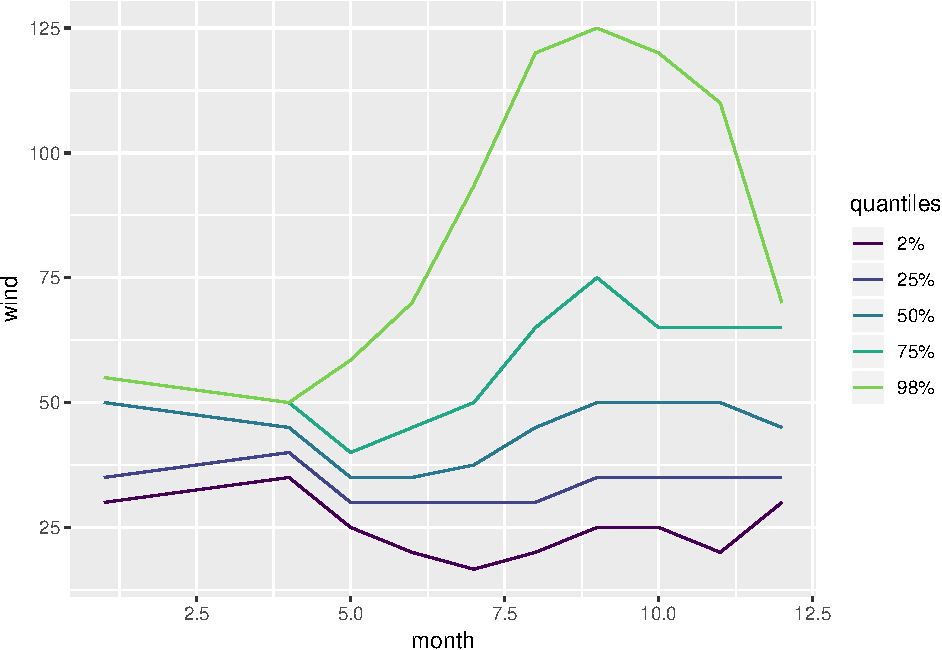
\includegraphics{R_tidyverse_for_geographers_files/figure-latex/dplyr::storms-6.pdf}

\hypertarget{pca-example-with-columns-scaling--}{%
\section{PCA example with columns scaling
-------------------------------------------------------------}\label{pca-example-with-columns-scaling--}}

\begin{Shaded}
\begin{Highlighting}[]
\CommentTok{# iris %>%}
  \CommentTok{# select(-Species) %>% }
  \CommentTok{# prcomp(~., data=.) %>% # BAD!, vars need to be scaled}
  \CommentTok{# biplot()}
\end{Highlighting}
\end{Shaded}

\begin{Shaded}
\begin{Highlighting}[]
\NormalTok{iris }\OperatorTok\StringTok{ }
\StringTok{  }\KeywordTok{group_by}\NormalTok{(Species) }\OperatorTok\StringTok{ }
\StringTok{  }\KeywordTok{mutate_all}\NormalTok{(scale) }\OperatorTok\StringTok{ }
\StringTok{  }\KeywordTok{prcomp}\NormalTok{(}\OperatorTok{~}\NormalTok{.}\OperatorTok{-}\NormalTok{Species, }\DataTypeTok{data=}\NormalTok{.) }\OperatorTok\StringTok{ }
\StringTok{  }\KeywordTok{biplot}\NormalTok{()}
\end{Highlighting}
\end{Shaded}

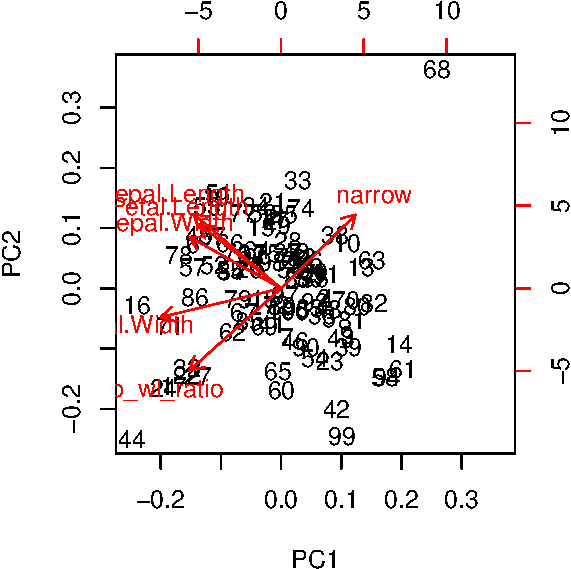
\includegraphics{R_tidyverse_for_geographers_files/figure-latex/unnamed-chunk-30-1.pdf}

\hypertarget{reshaping-data-example}{%
\section{Reshaping data example
--------------------------------------------------}\label{reshaping-data-example}}

\begin{Shaded}
\begin{Highlighting}[]
\NormalTok{population }\OperatorTok\StringTok{ }
\StringTok{  }\KeywordTok{filter}\NormalTok{(country}\OperatorTok{==}\StringTok{"Italy"}\NormalTok{) }\OperatorTok\StringTok{ }
\StringTok{  }\KeywordTok{ggplot}\NormalTok{(}\DataTypeTok{data=}\NormalTok{., }\KeywordTok{aes}\NormalTok{(year, population))}\OperatorTok{+}\KeywordTok{geom_line}\NormalTok{()}\OperatorTok{+}\KeywordTok{geom_point}\NormalTok{()}
\end{Highlighting}
\end{Shaded}

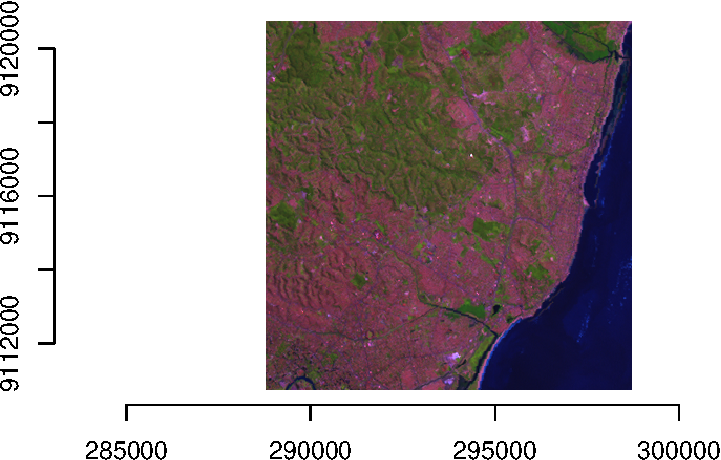
\includegraphics{R_tidyverse_for_geographers_files/figure-latex/unnamed-chunk-31-1.pdf}

\hypertarget{super-advanced-dplyr--}{%
\section{Super advanced dplyr
----------------------------------------------------}\label{super-advanced-dplyr--}}

\hypertarget{inspired-by-httpstwitter.comsuzanbaert-and-modified-from-httpsgithub.comsuzanbaertrladies_rocurblobmasterdplyr_tricks.pdf}{%
\section{\texorpdfstring{inspired by:
\url{https://twitter.com/SuzanBaert} and modified from:
\url{https://github.com/suzanbaert/RLadies_RoCur/blob/master/Dplyr_tricks.pdf}}{inspired by: https://twitter.com/SuzanBaert and modified from: https://github.com/suzanbaert/RLadies\_RoCur/blob/master/Dplyr\_tricks.pdf}}\label{inspired-by-httpstwitter.comsuzanbaert-and-modified-from-httpsgithub.comsuzanbaertrladies_rocurblobmasterdplyr_tricks.pdf}}

\begin{Shaded}
\begin{Highlighting}[]
\CommentTok{# using !! "bang"}
\NormalTok{vars <-}\StringTok{ }\KeywordTok{c}\NormalTok{(}\StringTok{"lat"}\NormalTok{,}\StringTok{"long"}\NormalTok{,}\StringTok{"wind"}\NormalTok{)}
\NormalTok{storms }\OperatorTok\StringTok{ }\KeywordTok{select}\NormalTok{(}\OperatorTok{!!}\NormalTok{vars)}
\end{Highlighting}
\end{Shaded}

\begin{verbatim}
## # A tibble: 10,010 x 3
##      lat  long  wind
##    <dbl> <dbl> <int>
##  1  27.5 -79      25
##  2  28.5 -79      25
##  3  29.5 -79      25
##  4  30.5 -79      25
##  5  31.5 -78.8    25
##  6  32.4 -78.7    25
##  7  33.3 -78      25
##  8  34   -77      30
##  9  34.4 -75.8    35
## 10  34   -74.8    40
## # ... with 10,000 more rows
\end{verbatim}

\begin{Shaded}
\begin{Highlighting}[]
\CommentTok{# select columns by regex}
\NormalTok{who }\OperatorTok\StringTok{ }\NormalTok{names }\CommentTok{# lots of column names}
\end{Highlighting}
\end{Shaded}

\begin{verbatim}
##  [1] "country"      "iso2"         "iso3"         "year"        
##  [5] "new_sp_m014"  "new_sp_m1524" "new_sp_m2534" "new_sp_m3544"
##  [9] "new_sp_m4554" "new_sp_m5564" "new_sp_m65"   "new_sp_f014" 
## [13] "new_sp_f1524" "new_sp_f2534" "new_sp_f3544" "new_sp_f4554"
## [17] "new_sp_f5564" "new_sp_f65"   "new_sn_m014"  "new_sn_m1524"
## [21] "new_sn_m2534" "new_sn_m3544" "new_sn_m4554" "new_sn_m5564"
## [25] "new_sn_m65"   "new_sn_f014"  "new_sn_f1524" "new_sn_f2534"
## [29] "new_sn_f3544" "new_sn_f4554" "new_sn_f5564" "new_sn_f65"  
## [33] "new_ep_m014"  "new_ep_m1524" "new_ep_m2534" "new_ep_m3544"
## [37] "new_ep_m4554" "new_ep_m5564" "new_ep_m65"   "new_ep_f014" 
## [41] "new_ep_f1524" "new_ep_f2534" "new_ep_f3544" "new_ep_f4554"
## [45] "new_ep_f5564" "new_ep_f65"   "newrel_m014"  "newrel_m1524"
## [49] "newrel_m2534" "newrel_m3544" "newrel_m4554" "newrel_m5564"
## [53] "newrel_m65"   "newrel_f014"  "newrel_f1524" "newrel_f2534"
## [57] "newrel_f3544" "newrel_f4554" "newrel_f5564" "newrel_f65"
\end{verbatim}

\begin{Shaded}
\begin{Highlighting}[]
\NormalTok{who }\OperatorTok\StringTok{ }\KeywordTok{select}\NormalTok{(country, year, }\KeywordTok{matches}\NormalTok{(}\StringTok{"*2534"}\NormalTok{)) }\CommentTok{# select country, year, and columns with '2534' in the name}
\end{Highlighting}
\end{Shaded}

\begin{verbatim}
## # A tibble: 7,240 x 10
##    country      year new_sp_m2534 new_sp_f2534 new_sn_m2534 new_sn_f2534
##    <chr>       <int>        <int>        <int>        <int>        <int>
##  1 Afghanistan  1980           NA           NA           NA           NA
##  2 Afghanistan  1981           NA           NA           NA           NA
##  3 Afghanistan  1982           NA           NA           NA           NA
##  4 Afghanistan  1983           NA           NA           NA           NA
##  5 Afghanistan  1984           NA           NA           NA           NA
##  6 Afghanistan  1985           NA           NA           NA           NA
##  7 Afghanistan  1986           NA           NA           NA           NA
##  8 Afghanistan  1987           NA           NA           NA           NA
##  9 Afghanistan  1988           NA           NA           NA           NA
## 10 Afghanistan  1989           NA           NA           NA           NA
## # ... with 7,230 more rows, and 4 more variables: new_ep_m2534 <int>,
## #   new_ep_f2534 <int>, newrel_m2534 <int>, newrel_f2534 <int>
\end{verbatim}

\begin{Shaded}
\begin{Highlighting}[]
\CommentTok{# rename columns with regex}
\KeywordTok{library}\NormalTok{(stringr);}
\NormalTok{iris }\OperatorTok\StringTok{ }
\StringTok{  }\KeywordTok{as_tibble}\NormalTok{() }\OperatorTok\StringTok{ }
\StringTok{  }\KeywordTok{rename_all}\NormalTok{(tolower) }\OperatorTok\StringTok{ }
\StringTok{  }\KeywordTok{rename_all}\NormalTok{(}\OperatorTok{~}\KeywordTok{str_replace_all}\NormalTok{(., }\StringTok{"}\CharTok{\textbackslash{}\textbackslash{}}\StringTok{."}\NormalTok{,}\StringTok{"_"}\NormalTok{))}
\end{Highlighting}
\end{Shaded}

\begin{verbatim}
## # A tibble: 150 x 7
##    sepal_length sepal_width petal_length petal_width species p_wl_ratio
##           <dbl>       <dbl>        <dbl>       <dbl> <fct>        <dbl>
##  1          5.1         3.5          1.4         0.2 setosa      0.143 
##  2          4.9         3            1.4         0.2 setosa      0.143 
##  3          4.7         3.2          1.3         0.2 setosa      0.154 
##  4          4.6         3.1          1.5         0.2 setosa      0.133 
##  5          5           3.6          1.4         0.2 setosa      0.143 
##  6          5.4         3.9          1.7         0.4 setosa      0.235 
##  7          4.6         3.4          1.4         0.3 setosa      0.214 
##  8          5           3.4          1.5         0.2 setosa      0.133 
##  9          4.4         2.9          1.4         0.2 setosa      0.143 
## 10          4.9         3.1          1.5         0.1 setosa      0.0667
## # ... with 140 more rows, and 1 more variable: narrow <lgl>
\end{verbatim}

\begin{Shaded}
\begin{Highlighting}[]
\CommentTok{# mutate *observation* names}
\NormalTok{storms }\OperatorTok\StringTok{ }
\StringTok{  }\KeywordTok{select}\NormalTok{(name,year,status) }\OperatorTok\StringTok{ }
\StringTok{  }\KeywordTok{mutate_all}\NormalTok{(tolower) }\OperatorTok\StringTok{ }\CommentTok{# Amy -> amy}
\StringTok{  }\KeywordTok{mutate_all}\NormalTok{(}\OperatorTok{~}\KeywordTok{str_replace_all}\NormalTok{(., }\StringTok{" "}\NormalTok{,}\StringTok{"_"}\NormalTok{)) }\CommentTok{# 'tropical depression' -> 'tropical_depression'}
\end{Highlighting}
\end{Shaded}

\begin{verbatim}
## # A tibble: 10,010 x 3
##    name  year  status             
##    <chr> <chr> <chr>              
##  1 amy   1975  tropical_depression
##  2 amy   1975  tropical_depression
##  3 amy   1975  tropical_depression
##  4 amy   1975  tropical_depression
##  5 amy   1975  tropical_depression
##  6 amy   1975  tropical_depression
##  7 amy   1975  tropical_depression
##  8 amy   1975  tropical_depression
##  9 amy   1975  tropical_storm     
## 10 amy   1975  tropical_storm     
## # ... with 10,000 more rows
\end{verbatim}

\begin{Shaded}
\begin{Highlighting}[]
\CommentTok{# find highest values}
\NormalTok{storms }\OperatorTok\StringTok{ }
\StringTok{  }\KeywordTok{top_n}\NormalTok{(}\DecValTok{5}\NormalTok{, wind) }\CommentTok{# storms with 5 highest windspeeds}
\end{Highlighting}
\end{Shaded}

\begin{verbatim}
## # A tibble: 7 x 13
##   name   year month   day  hour   lat  long status category  wind pressure
##   <chr> <dbl> <dbl> <int> <dbl> <dbl> <dbl> <chr>  <ord>    <int>    <int>
## 1 Gilb~  1988     9    14     0  19.7 -83.8 hurri~ 5          160      888
## 2 Gilb~  1988     9    14     6  19.9 -85.3 hurri~ 5          155      889
## 3 Mitch  1998    10    26    18  16.9 -83.1 hurri~ 5          155      905
## 4 Mitch  1998    10    27     0  17.2 -83.8 hurri~ 5          155      910
## 5 Rita   2005     9    22     3  24.7 -87.3 hurri~ 5          155      895
## 6 Rita   2005     9    22     6  24.8 -87.6 hurri~ 5          155      897
## 7 Wilma  2005    10    19    12  17.3 -82.8 hurri~ 5          160      882
## # ... with 2 more variables: ts_diameter <dbl>, hu_diameter <dbl>
\end{verbatim}

\begin{Shaded}
\begin{Highlighting}[]
\CommentTok{# making new vars from conditions}
\NormalTok{starwars }\OperatorTok
\StringTok{  }\KeywordTok{select}\NormalTok{(name, species, homeworld, birth_year, hair_color) }\OperatorTok
\StringTok{  }\KeywordTok{mutate}\NormalTok{(}\DataTypeTok{new_group =} \KeywordTok{case_when}\NormalTok{(}
\NormalTok{    species }\OperatorTok{==}\StringTok{ "Droid"} \OperatorTok{~}\StringTok{ "Robot"}\NormalTok{,}
\NormalTok{    homeworld }\OperatorTok{==}\StringTok{ "Tatooine"} \OperatorTok{&}\StringTok{ }\NormalTok{hair_color }\OperatorTok{==}\StringTok{ "blond"} \OperatorTok{~}\StringTok{ "Blond Tatooinian"}\NormalTok{,}
\NormalTok{    homeworld }\OperatorTok{==}\StringTok{ "Tatooine"} \OperatorTok{~}\StringTok{ "Other Tatooinian"}\NormalTok{,}
\NormalTok{    hair_color }\OperatorTok{==}\StringTok{ "blond"} \OperatorTok{~}\StringTok{ "Blond non-Tatooinian"}\NormalTok{,}
    \OtherTok{TRUE} \OperatorTok{~}\StringTok{ "Other Human"}\NormalTok{))}
\end{Highlighting}
\end{Shaded}

\begin{verbatim}
## # A tibble: 87 x 6
##    name               species homeworld birth_year hair_color    new_group
##    <chr>              <chr>   <chr>          <dbl> <chr>         <chr>    
##  1 Luke Skywalker     Human   Tatooine        19   blond         Blond Ta~
##  2 C-3PO              Droid   Tatooine       112   <NA>          Robot    
##  3 R2-D2              Droid   Naboo           33   <NA>          Robot    
##  4 Darth Vader        Human   Tatooine        41.9 none          Other Ta~
##  5 Leia Organa        Human   Alderaan        19   brown         Other Hu~
##  6 Owen Lars          Human   Tatooine        52   brown, grey   Other Ta~
##  7 Beru Whitesun lars Human   Tatooine        47   brown         Other Ta~
##  8 R5-D4              Droid   Tatooine        NA   <NA>          Robot    
##  9 Biggs Darklighter  Human   Tatooine        24   black         Other Ta~
## 10 Obi-Wan Kenobi     Human   Stewjon         57   auburn, white Other Hu~
## # ... with 77 more rows
\end{verbatim}

\hypertarget{spatial-methods-tidyverse}{%
\section{SPATIAL METHODS + TIDYVERSE
---------------------------------------------}\label{spatial-methods-tidyverse}}

\begin{Shaded}
\begin{Highlighting}[]
\CommentTok{# Required libraries: }
\KeywordTok{library}\NormalTok{(sf); }
\end{Highlighting}
\end{Shaded}

\begin{verbatim}
## Linking to GEOS 3.5.0, GDAL 2.1.3, proj.4 4.9.2
\end{verbatim}

\begin{Shaded}
\begin{Highlighting}[]
\KeywordTok{library}\NormalTok{(tidyverse); }
\KeywordTok{library}\NormalTok{(lubridate); }

\KeywordTok{dir.create}\NormalTok{(}\StringTok{"data/SouthAmerica"}\NormalTok{)}
\end{Highlighting}
\end{Shaded}

\begin{verbatim}
## Warning in dir.create("data/SouthAmerica"): 'data/SouthAmerica' already
## exists
\end{verbatim}

\begin{Shaded}
\begin{Highlighting}[]
\KeywordTok{unzip}\NormalTok{(}\DataTypeTok{zipfile =} \StringTok{"data/SouthAmerica.zip"}\NormalTok{, }\DataTypeTok{exdir =} \StringTok{"data/SouthAmerica"}\NormalTok{)}
\KeywordTok{list.files}\NormalTok{(}\StringTok{'data/SouthAmerica/'}\NormalTok{)}
\end{Highlighting}
\end{Shaded}

\begin{verbatim}
## [1] "SouthAmerica.dbf"     "SouthAmerica.prj"     "SouthAmerica.sbn"    
## [4] "SouthAmerica.sbx"     "SouthAmerica.shp"     "SouthAmerica.shp.xml"
## [7] "SouthAmerica.shx"
\end{verbatim}

\begin{Shaded}
\begin{Highlighting}[]
\NormalTok{SA <-}\StringTok{ }\NormalTok{sf}\OperatorTok{::}\KeywordTok{st_read}\NormalTok{(}\StringTok{"data/SouthAmerica/SouthAmerica.shp"}\NormalTok{)}
\end{Highlighting}
\end{Shaded}

\begin{verbatim}
## Reading layer `SouthAmerica' from data source `/home/sami/srifai@gmail.com/work/Teaching/R_for_geographers/data/SouthAmerica/SouthAmerica.shp' using driver `ESRI Shapefile'
## Simple feature collection with 15 features and 18 fields
## geometry type:  MULTIPOLYGON
## dimension:      XY
## bbox:           xmin: -10192560 ymin: -7508478 xmax: -3868796 ymax: 1396462
## epsg (SRID):    NA
## proj4string:    +proj=merc +lon_0=0 +lat_ts=0 +x_0=0 +y_0=0 +a=6371000 +b=6371000 +units=m +no_defs
\end{verbatim}

\begin{Shaded}
\begin{Highlighting}[]
\KeywordTok{plot}\NormalTok{(SA) }\CommentTok{# blah, not ideal}
\end{Highlighting}
\end{Shaded}

\begin{verbatim}
## Warning: plotting the first 10 out of 18 attributes; use max.plot = 18 to
## plot all
\end{verbatim}

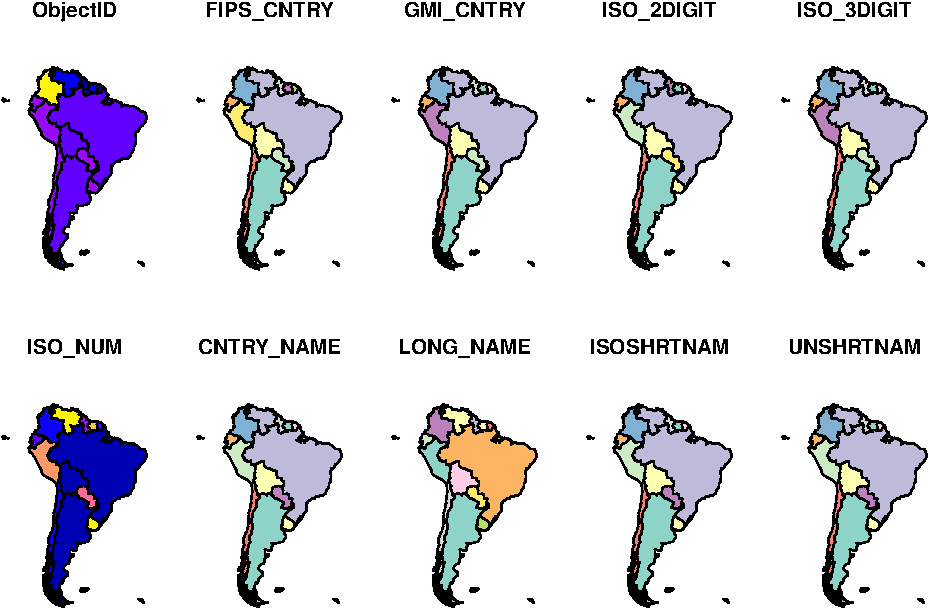
\includegraphics{R_tidyverse_for_geographers_files/figure-latex/unnamed-chunk-33-1.pdf}

\begin{Shaded}
\begin{Highlighting}[]
\KeywordTok{plot}\NormalTok{(SA[}\StringTok{"SQKM"}\NormalTok{]) }\CommentTok{# base R method - a little better, but not so easy to control}
\end{Highlighting}
\end{Shaded}

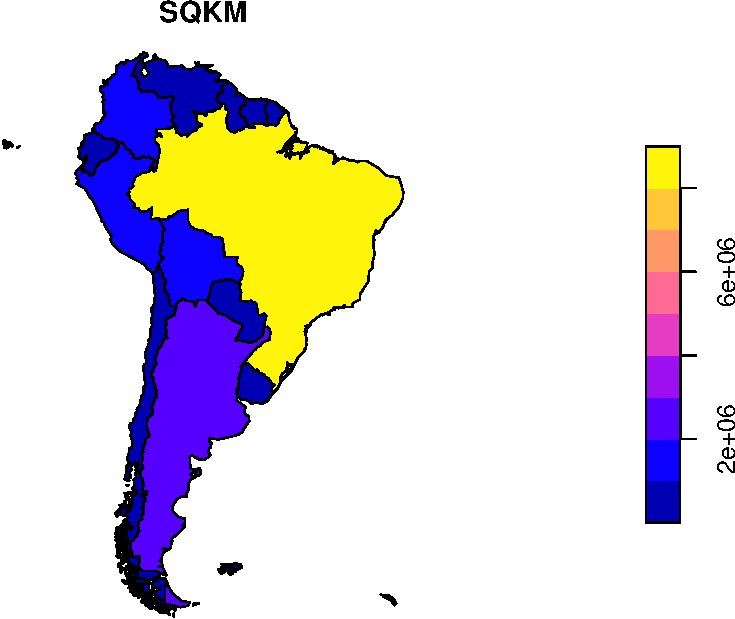
\includegraphics{R_tidyverse_for_geographers_files/figure-latex/unnamed-chunk-33-2.pdf}

\begin{Shaded}
\begin{Highlighting}[]
\KeywordTok{ggplot}\NormalTok{() }\OperatorTok{+}\StringTok{ }\KeywordTok{geom_sf}\NormalTok{(}\DataTypeTok{data=}\NormalTok{SA, }\KeywordTok{aes}\NormalTok{(}\DataTypeTok{fill=}\NormalTok{SQKM))}\OperatorTok{+}
\StringTok{  }\KeywordTok{scale_fill_viridis_c}\NormalTok{()}
\end{Highlighting}
\end{Shaded}

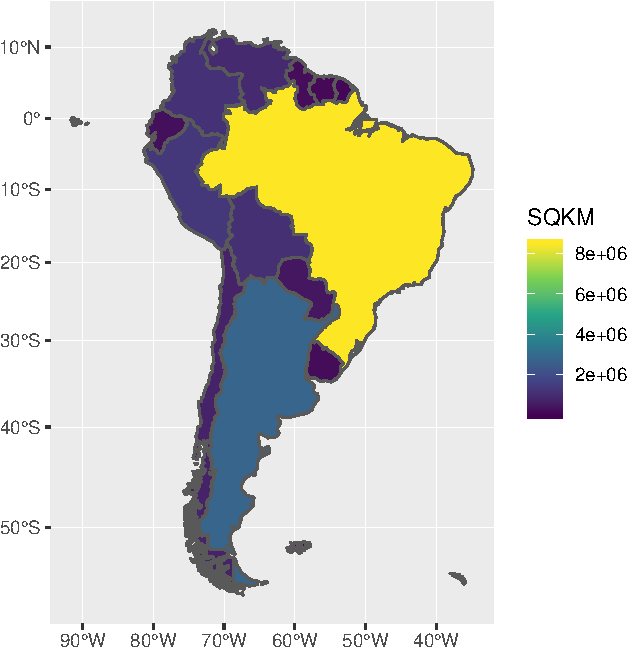
\includegraphics{R_tidyverse_for_geographers_files/figure-latex/unnamed-chunk-33-3.pdf}

\begin{Shaded}
\begin{Highlighting}[]
\KeywordTok{ggplot}\NormalTok{() }\OperatorTok{+}\StringTok{ }\KeywordTok{geom_sf}\NormalTok{(}\DataTypeTok{data=}\NormalTok{SA, }\KeywordTok{aes}\NormalTok{(}\DataTypeTok{fill=}\KeywordTok{log}\NormalTok{(SQKM, }\DataTypeTok{base =} \DecValTok{10}\NormalTok{)))}\OperatorTok{+}
\StringTok{  }\KeywordTok{scale_fill_viridis_c}\NormalTok{()}
\end{Highlighting}
\end{Shaded}

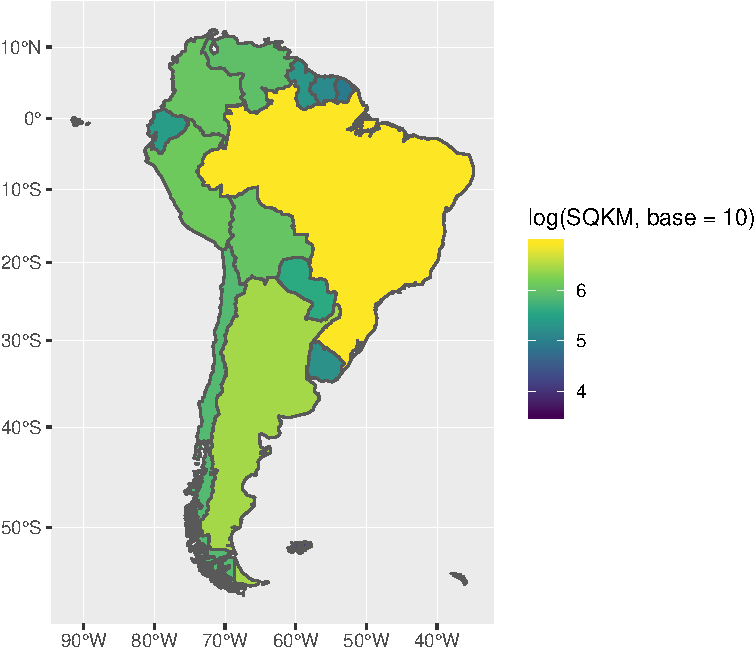
\includegraphics{R_tidyverse_for_geographers_files/figure-latex/unnamed-chunk-33-4.pdf}

\begin{Shaded}
\begin{Highlighting}[]
\CommentTok{# SA %>% mutate(population=ifelse(POP2007>0, POP2007,1)) %>% }
\CommentTok{#   select(population) %>% pull(population)}
\CommentTok{#   ggplot()+}
\CommentTok{#   geom_sf(data=SA, aes(fill=population))+}
\CommentTok{#   scale_fill_viridis_c()}



\CommentTok{# SA %>% }
\CommentTok{#   ggplot(data=., aes())+geom_sf(fill="SQKM")+}
\CommentTok{#   geom_point(data=data.frame(lat=0,lon=-80),aes(lat,lon),col='red')}
\CommentTok{# }
\CommentTok{# ggplot(data=SA, aes())+geom_sf()+}
\CommentTok{#   geom_point(data=data.frame(lat=0,lon=-80),aes(lat,lon),col='red')}
\end{Highlighting}
\end{Shaded}

\begin{Shaded}
\begin{Highlighting}[]
\KeywordTok{library}\NormalTok{(tidyverse)}
\CommentTok{# Calculate NDVI from Landsat 7 -------------------------------------------}
\NormalTok{tif =}\StringTok{ }\KeywordTok{system.file}\NormalTok{(}\StringTok{"tif/L7_ETMs.tif"}\NormalTok{, }\DataTypeTok{package =} \StringTok{"stars"}\NormalTok{)}
\NormalTok{(}\DataTypeTok{r =}\NormalTok{ raster}\OperatorTok{::}\KeywordTok{stack}\NormalTok{(tif))}
\end{Highlighting}
\end{Shaded}

\begin{verbatim}
## class       : RasterStack 
## dimensions  : 352, 349, 122848, 6  (nrow, ncol, ncell, nlayers)
## resolution  : 28.5, 28.5  (x, y)
## extent      : 288776.3, 298722.8, 9110729, 9120761  (xmin, xmax, ymin, ymax)
## coord. ref. : +proj=utm +zone=25 +south +ellps=GRS80 +towgs84=0,0,0,0,0,0,0 +units=m +no_defs 
## names       : L7_ETMs.1, L7_ETMs.2, L7_ETMs.3, L7_ETMs.4, L7_ETMs.5, L7_ETMs.6 
## min values  :         0,         0,         0,         0,         0,         0 
## max values  :       255,       255,       255,       255,       255,       255
\end{verbatim}

\begin{Shaded}
\begin{Highlighting}[]
\NormalTok{raster}\OperatorTok{::}\KeywordTok{plot}\NormalTok{(r) }\CommentTok{# Not ideal.}
\end{Highlighting}
\end{Shaded}

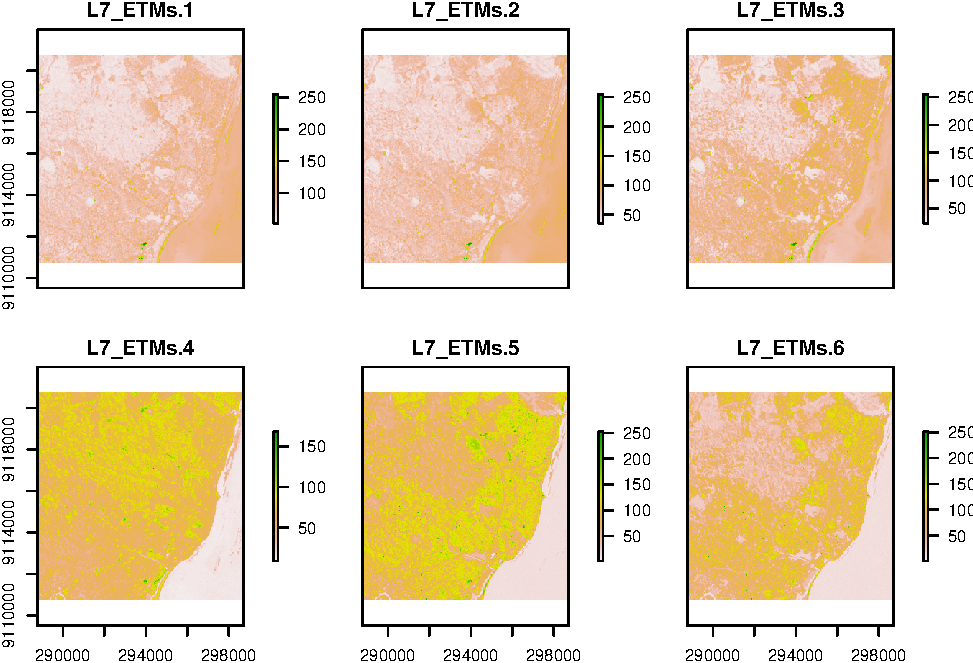
\includegraphics{R_tidyverse_for_geographers_files/figure-latex/unnamed-chunk-34-1.pdf}

\begin{Shaded}
\begin{Highlighting}[]
\NormalTok{l7 <-}\StringTok{ }\NormalTok{raster}\OperatorTok{::}\KeywordTok{as.data.frame}\NormalTok{(r, }\DataTypeTok{xy=}\NormalTok{T) }\OperatorTok\StringTok{ }\KeywordTok{as_tibble}\NormalTok{()}
\NormalTok{l7 <-}\StringTok{ }\NormalTok{l7 }\OperatorTok
\StringTok{  }\KeywordTok{mutate}\NormalTok{(}\DataTypeTok{ndvi=}\NormalTok{(L7_ETMs}\FloatTok{.4}\OperatorTok{-}\NormalTok{L7_ETMs}\FloatTok{.3}\NormalTok{)}\OperatorTok{/}\NormalTok{(L7_ETMs}\FloatTok{.4}\OperatorTok{+}\NormalTok{L7_ETMs}\FloatTok{.3}\NormalTok{))}
\NormalTok{l7 }\OperatorTok\StringTok{ }
\StringTok{  }\KeywordTok{ggplot}\NormalTok{(}\DataTypeTok{data=}\NormalTok{., }\KeywordTok{aes}\NormalTok{(x,y,}\DataTypeTok{fill=}\NormalTok{ndvi))}\OperatorTok{+}
\StringTok{  }\KeywordTok{geom_raster}\NormalTok{()}\OperatorTok{+}
\StringTok{  }\KeywordTok{coord_equal}\NormalTok{()}\OperatorTok{+}
\StringTok{  }\KeywordTok{theme_bw}\NormalTok{()}\OperatorTok{+}
\StringTok{  }\KeywordTok{scale_fill_viridis_c}\NormalTok{(}\StringTok{"NDVI"}\NormalTok{)}\OperatorTok{+}
\StringTok{  }\KeywordTok{labs}\NormalTok{(}\DataTypeTok{x=}\StringTok{"UTM X [m]"}\NormalTok{,}\DataTypeTok{y=}\StringTok{"UTM Y [m]"}\NormalTok{)}\OperatorTok{+}
\StringTok{  }\KeywordTok{theme}\NormalTok{(}\DataTypeTok{legend.position =} \KeywordTok{c}\NormalTok{(}\FloatTok{0.9}\NormalTok{,}\FloatTok{0.15}\NormalTok{),}
        \DataTypeTok{legend.title =} \KeywordTok{element_text}\NormalTok{(}\DataTypeTok{size=}\DecValTok{15}\NormalTok{, }\DataTypeTok{face =} \StringTok{'bold'}\NormalTok{),}
        \DataTypeTok{legend.text =} \KeywordTok{element_text}\NormalTok{(}\DataTypeTok{size=}\DecValTok{10}\NormalTok{),}
        \DataTypeTok{axis.title.x =} \KeywordTok{element_text}\NormalTok{(}\DataTypeTok{size=}\DecValTok{25}\NormalTok{), }
        \DataTypeTok{axis.text.x =} \KeywordTok{element_text}\NormalTok{(}\DataTypeTok{size=}\DecValTok{15}\NormalTok{), }
        \DataTypeTok{axis.title.y =} \KeywordTok{element_text}\NormalTok{(}\DataTypeTok{size=}\DecValTok{25}\NormalTok{), }
        \DataTypeTok{axis.text.y =} \KeywordTok{element_text}\NormalTok{(}\DataTypeTok{size=}\DecValTok{15}\NormalTok{))}
\end{Highlighting}
\end{Shaded}

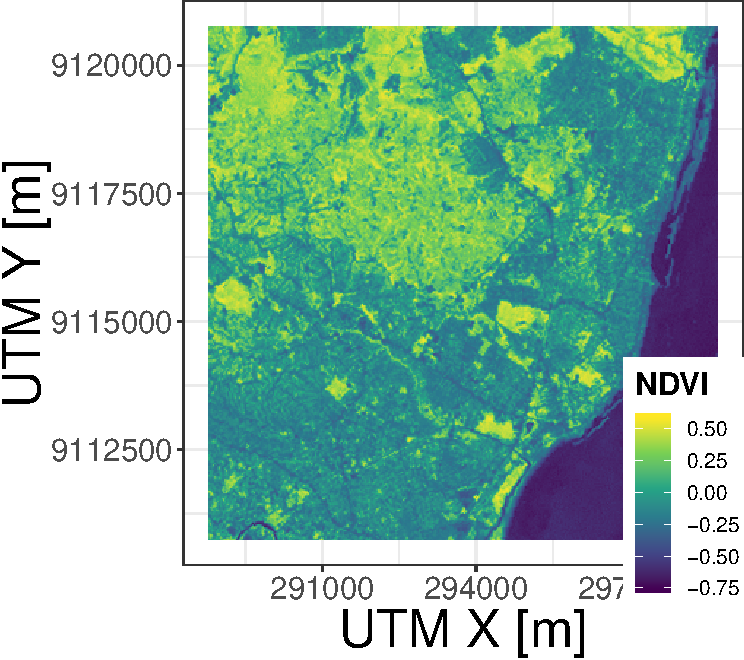
\includegraphics{R_tidyverse_for_geographers_files/figure-latex/unnamed-chunk-34-2.pdf}

\hypertarget{a-peak-into-stars}{%
\section{A peak into stars!
------------------------------------------------------------------}\label{a-peak-into-stars}}

\hypertarget{stars-is-developing-package-for-dealing-with-spatial-raster-and-vector-data}{%
\section{stars is developing package for dealing with spatial raster and
vector
data}\label{stars-is-developing-package-for-dealing-with-spatial-raster-and-vector-data}}

\hypertarget{its-tidyverse-compliant-and-iswill-be-much-better-suited-for-processing-large-spatial-data-in-r}{%
\section{It's tidyverse compliant, and is/will be much better suited for
processing large spatial data in
R}\label{its-tidyverse-compliant-and-iswill-be-much-better-suited-for-processing-large-spatial-data-in-r}}

\#{[}\url{https://www.r-spatial.org/r/2018/03/22/stars2.html}{]}

\#! CAUTIONARY NOTE ! if you are processing Gbs worth of raster or other
spatiotemporal data, consider doing it in Python

\begin{Shaded}
\begin{Highlighting}[]
\KeywordTok{library}\NormalTok{(stars)}
\end{Highlighting}
\end{Shaded}

\begin{verbatim}
## Loading required package: abind
\end{verbatim}

\begin{Shaded}
\begin{Highlighting}[]
\NormalTok{tif =}\StringTok{ }\KeywordTok{system.file}\NormalTok{(}\StringTok{"tif/L7_ETMs.tif"}\NormalTok{, }\DataTypeTok{package =} \StringTok{"stars"}\NormalTok{)}
\NormalTok{(}\DataTypeTok{r =}\NormalTok{ raster}\OperatorTok{::}\KeywordTok{stack}\NormalTok{(tif))}
\end{Highlighting}
\end{Shaded}

\begin{verbatim}
## class       : RasterStack 
## dimensions  : 352, 349, 122848, 6  (nrow, ncol, ncell, nlayers)
## resolution  : 28.5, 28.5  (x, y)
## extent      : 288776.3, 298722.8, 9110729, 9120761  (xmin, xmax, ymin, ymax)
## coord. ref. : +proj=utm +zone=25 +south +ellps=GRS80 +towgs84=0,0,0,0,0,0,0 +units=m +no_defs 
## names       : L7_ETMs.1, L7_ETMs.2, L7_ETMs.3, L7_ETMs.4, L7_ETMs.5, L7_ETMs.6 
## min values  :         0,         0,         0,         0,         0,         0 
## max values  :       255,       255,       255,       255,       255,       255
\end{verbatim}

\begin{Shaded}
\begin{Highlighting}[]
\NormalTok{raster}\OperatorTok{::}\KeywordTok{plot}\NormalTok{(r) }\CommentTok{# Not ideal.}
\end{Highlighting}
\end{Shaded}

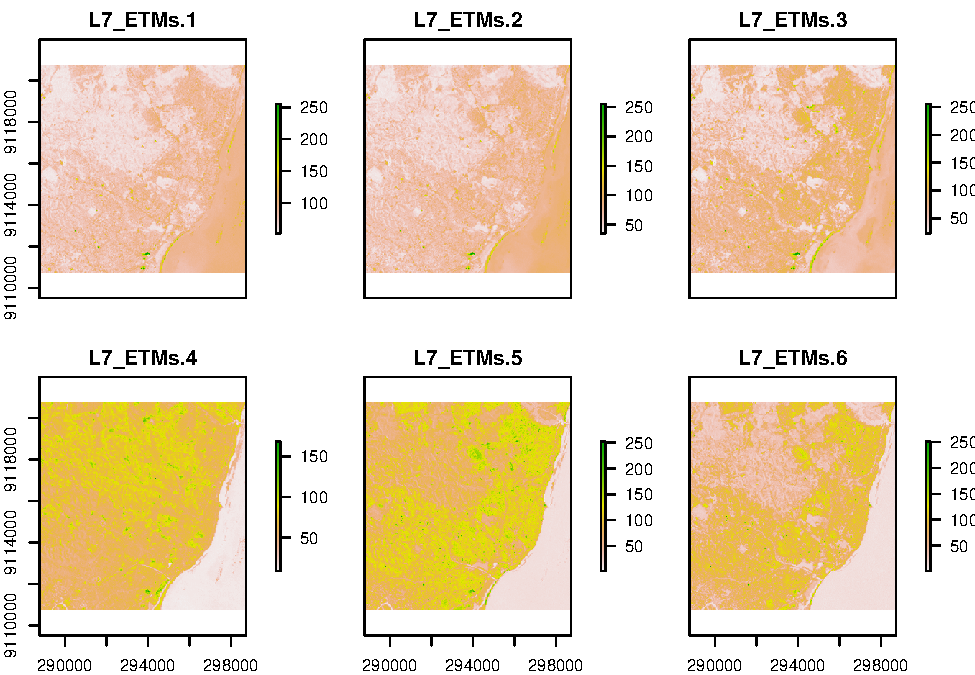
\includegraphics{R_tidyverse_for_geographers_files/figure-latex/unnamed-chunk-35-1.pdf}

\begin{Shaded}
\begin{Highlighting}[]
\NormalTok{(}\DataTypeTok{x =} \KeywordTok{read_stars}\NormalTok{(tif))}
\end{Highlighting}
\end{Shaded}

\begin{verbatim}
## stars object with 3 dimensions and 1 attribute
## attribute(s):
##   L7_ETMs.tif    
##  Min.   :  1.00  
##  1st Qu.: 54.00  
##  Median : 69.00  
##  Mean   : 68.91  
##  3rd Qu.: 86.00  
##  Max.   :255.00  
## dimension(s):
##      from  to  offset delta                       refsys point values
## x       1 349  288776  28.5 +proj=utm +zone=25 +south... FALSE   NULL
## y       1 352 9120761 -28.5 +proj=utm +zone=25 +south... FALSE   NULL
## band    1   6      NA    NA                           NA    NA   NULL
\end{verbatim}

\begin{Shaded}
\begin{Highlighting}[]
\KeywordTok{plot}\NormalTok{(x) }\CommentTok{# much improved (see ?plot.stars)}
\end{Highlighting}
\end{Shaded}

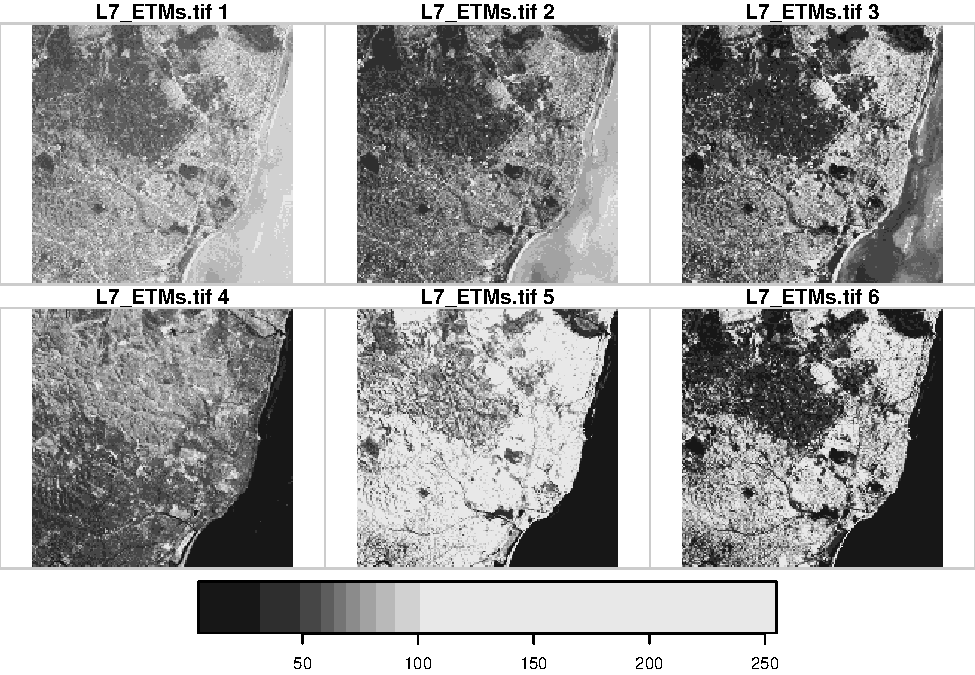
\includegraphics{R_tidyverse_for_geographers_files/figure-latex/unnamed-chunk-35-2.pdf}

\begin{Shaded}
\begin{Highlighting}[]
\NormalTok{x[,,,}\DecValTok{1}\NormalTok{] }\OperatorTok\StringTok{ }\NormalTok{plot }\CommentTok{# plot band 1}
\end{Highlighting}
\end{Shaded}

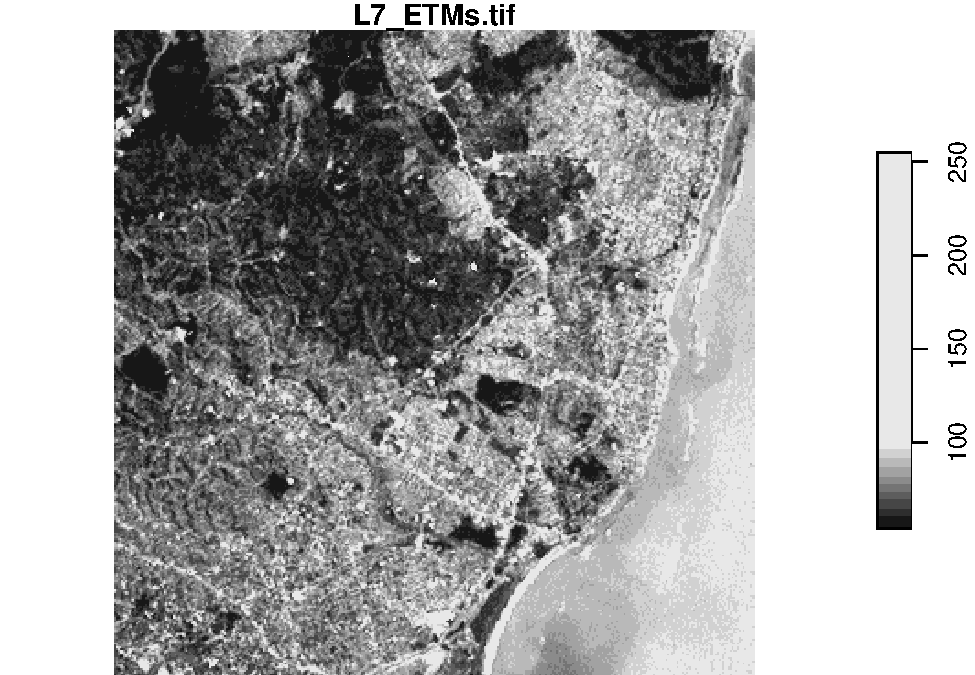
\includegraphics{R_tidyverse_for_geographers_files/figure-latex/unnamed-chunk-35-3.pdf}

\begin{Shaded}
\begin{Highlighting}[]
\NormalTok{x[,,,}\DecValTok{2}\NormalTok{] }\OperatorTok\StringTok{ }\NormalTok{plot }\CommentTok{# plot band 2}
\end{Highlighting}
\end{Shaded}

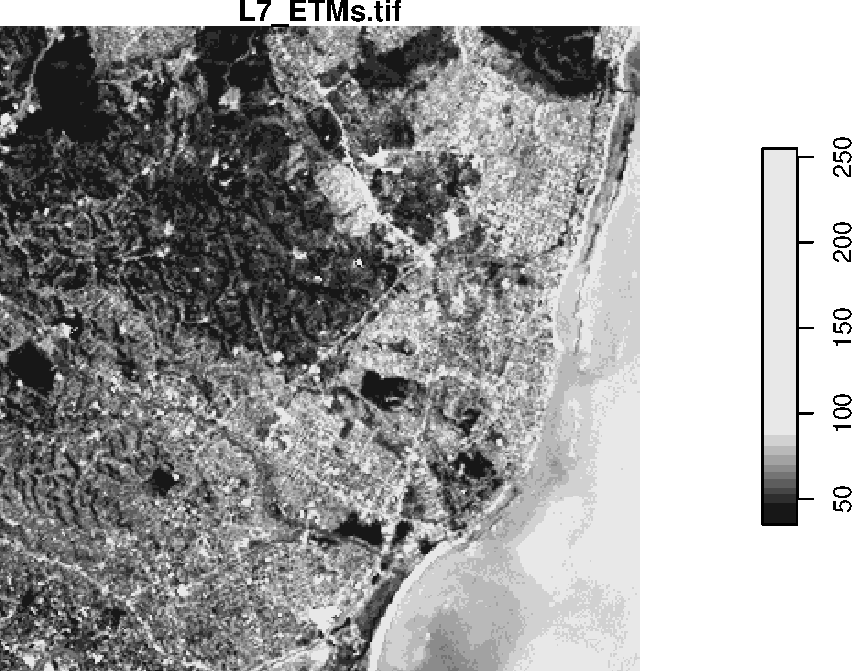
\includegraphics{R_tidyverse_for_geographers_files/figure-latex/unnamed-chunk-35-4.pdf}

\begin{Shaded}
\begin{Highlighting}[]
\NormalTok{x[,}\DecValTok{1}\OperatorTok{:}\DecValTok{100}\NormalTok{,}\DecValTok{1}\OperatorTok{:}\DecValTok{100}\NormalTok{,}\DecValTok{1}\NormalTok{] }\OperatorTok\StringTok{ }\NormalTok{plot }\CommentTok{# plot spatial subset}
\end{Highlighting}
\end{Shaded}

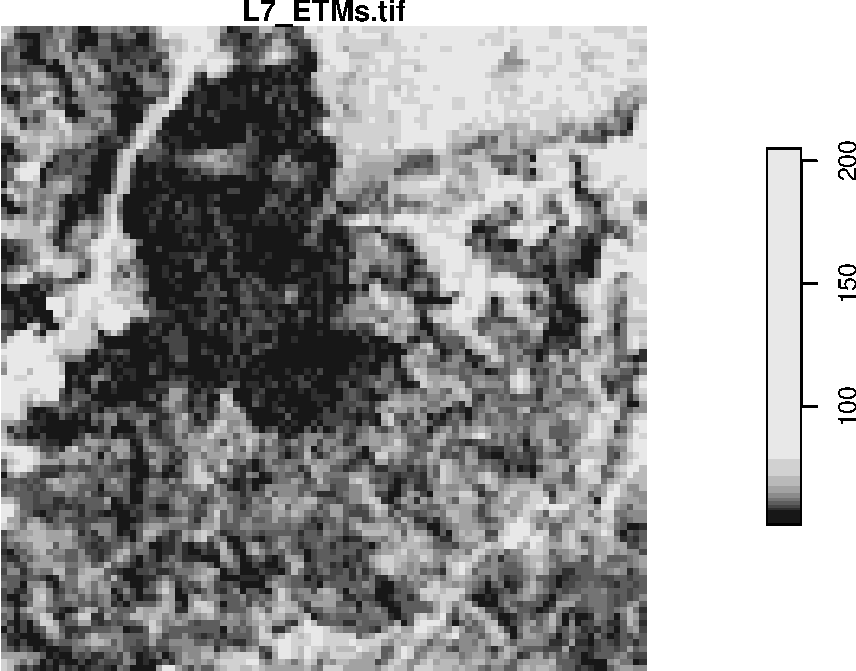
\includegraphics{R_tidyverse_for_geographers_files/figure-latex/unnamed-chunk-35-5.pdf}

\begin{Shaded}
\begin{Highlighting}[]
\NormalTok{x[,}\DecValTok{1}\OperatorTok{:}\DecValTok{10}\NormalTok{,}\DecValTok{1}\OperatorTok{:}\DecValTok{10}\NormalTok{,}\KeywordTok{c}\NormalTok{(}\DecValTok{1}\NormalTok{,}\DecValTok{2}\NormalTok{,}\DecValTok{3}\NormalTok{)] }\OperatorTok\StringTok{ }\NormalTok{plot}
\end{Highlighting}
\end{Shaded}

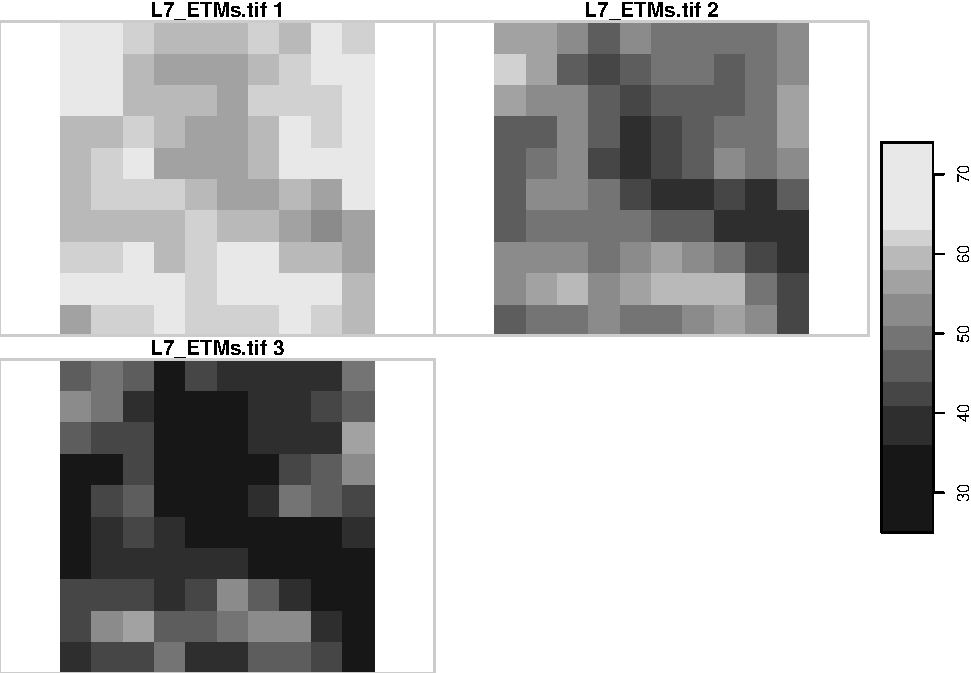
\includegraphics{R_tidyverse_for_geographers_files/figure-latex/unnamed-chunk-35-6.pdf}


\end{document}
